% EPL master thesis covers template
\documentclass{resources/EPL-master-thesis-covers-EN}
\usepackage[
  pdftex,
  pdfauthor={Guillaume Everarts de Velp},
  pdftitle={Improving the performance and the scalability of INGINIOUS},
  pdfsubject={Master thesis manuscript},
  pdfkeywords={Containerization, Docker, Virtualization}
]{hyperref}
\usepackage{tablefootnote}
\usepackage{longtable}
\usepackage{array}
\usepackage{subcaption}
\usepackage{dirtytalk}
\captionsetup[sub]{font=scriptsize}

% Please fill in the following boxes
% Title of the thesis
\title{Improving the performance and the scalability of INGINIOUS}

% Name of the student author(s)
\author{Guillaume \textsc{Everarts de Velp}}

% Official title of the master degree
\degreetitle{Master [120] in Computer Science and Engineering}

% Name of the supervisor(s)
\supervisor{Ramin \textsc{Sadre}}

% Name of the reader(s)
\readerone{Olivier \textsc{Bonaventure}}
\readertwo{Anthony \textsc{Gégo}}

% Academic year (update if necessary)
\years{2019--2020}

% Document
\begin{document}
  % Front cover page
  \maketitle
  
  \chapter*{Acknowledgements}

\paragraph{}A thesis is not a one man job, this one has been made possible thanks to the intervention of many people.  My deepest thanks go to my promoter, Professor Ramin Sadre, who guided me along this long project, providing support and advices and taking all the time required to do so accordingly.  A special thanks goes also to Professor Etienne Riviere who showed great interest in my work, and provided valuable advices.

\paragraph{}Of course this project wouldn't even have seen a day if Professor Olivier Bonaventure didn't talk me into it initially, it made me discover a new world, for this I am very grateful.  Thanks also to Anthony Gego for answering my numerous questions relatives to INGInious, to Mathieu Jadin for helping me in my first steps with cgroupv2, to Guillaume Rosinosky for setting me up an access to one of UCL's nuc.  Outside of the UCL other people helped me too, thanks to Corentin Badot-Bertrand for introducing me to Ansible, thanks to the \textit{Kata Containers} community and to the \textit{containers} organization for helping me with different issues.

\paragraph{}And finally, I would like to thank my family and friends for supporting me throughout this project, showing interest and offering support by all times. 

\begin{flushright}
  Guillaume Everarts de Velp, 2020
\end{flushright}

  \newpage
\begin{center}
  \section*{Abstract}
\end{center}

I studied different containerization solutions available, in different configurations, with the goal of determining the most appropriate one for INGInious.  That solution would be the one that can provide the best responsiveness while meeting the safety requirement that the platform has.  Based on my observations, I then present what would be the ideal solution for INGInious, with its performance gain over the best currently available solution and its drawbacks.  Finally, I address the performance cost of enforcing the isolation level, as some solutions offer, and the opportunities it brings to the platform.

  
  \tableofcontents
  
  \chapter{Introduction}

In this chapter I will simply introduce the subject of this master thesis, showing some basic concepts related to it and some key aspects.

\section{INGInious}

INGInious is a web platform developped by the UCL.  It is a tool for automatic correction of programs written by students.  It currently relies on Docker containers to provide a good isolation between the machine hosting the site and the execution of the student's codes.  So that a problem in a program submitted by a student couldn't have any impact on the platform.  Docker also allow to manage the resources granted to each code execution.  For now INGInious can meet the demand and provide honest performances and responsiveness.  But looking at the growing usage of the platform, we might soon come to a point where we reach the limits of the current implementation.

\subsection{Architecture}
INGInious counts four main components:
\begin{enumerate}
  \item The front-end: the website with which each student interacts when submitting a task.
  \item The back-end: a queue of all the tasks that need to be graded.
  \item The docker agent: responsible for the container assignment to the pending tasks when resources are available.
  \item The docker containers: one for the student code and one for the teacher tests evaluating the student's code behaviour.
\end{enumerate}
The journey of a task submitted on INGInious is represented on Figure \ref{fig:architecture}.
\begin{figure}[!h]
  \begin{center}
    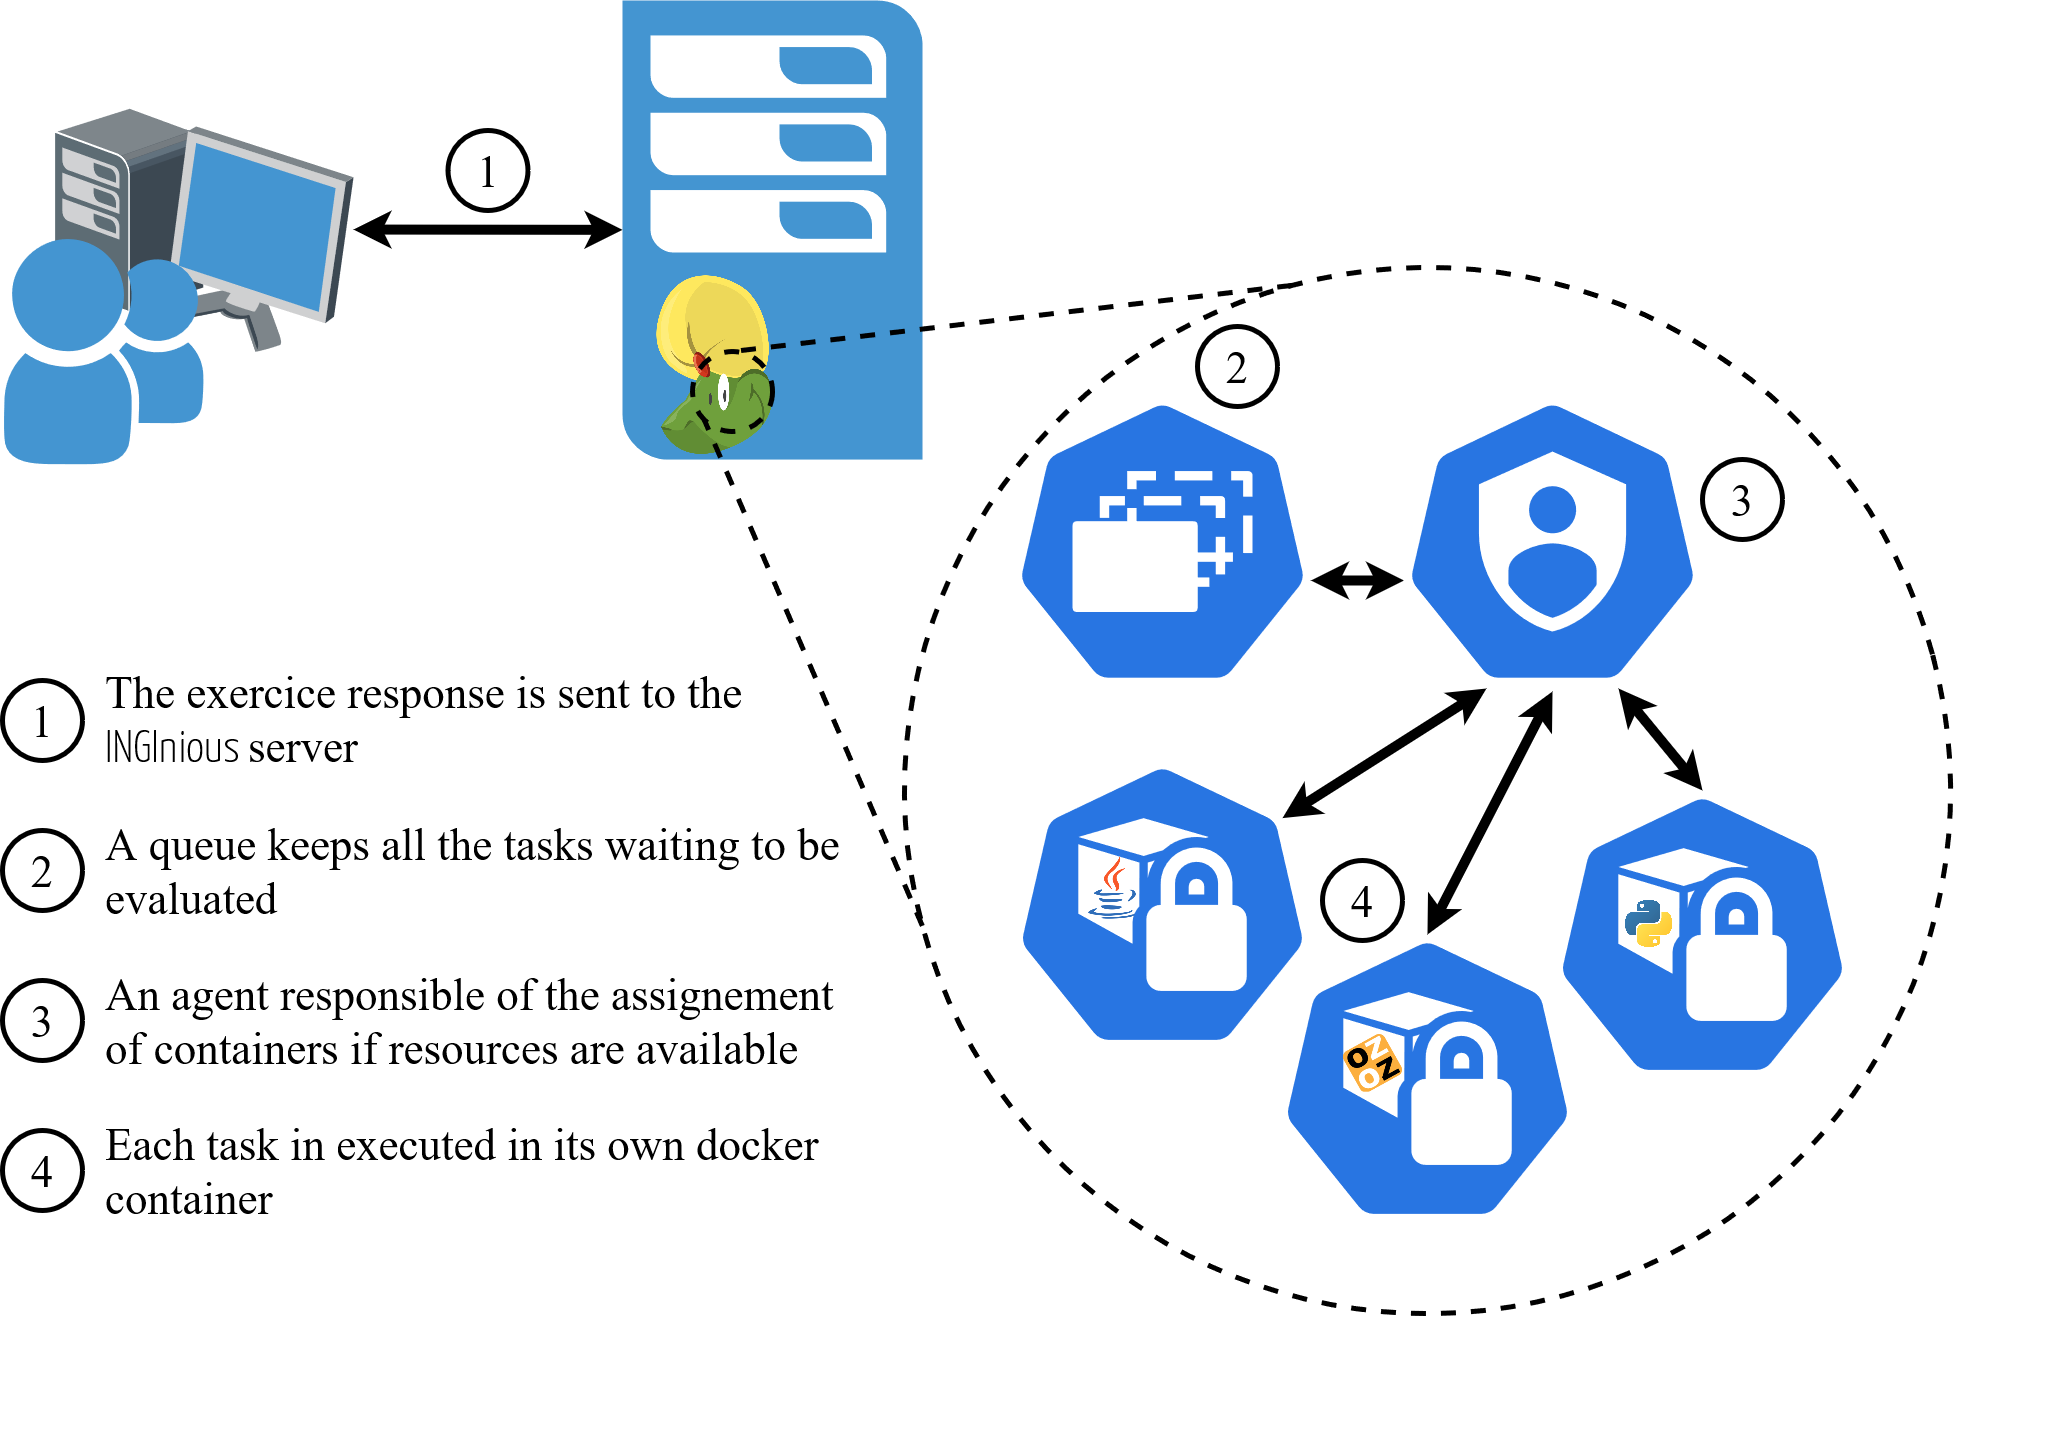
\includegraphics[width=\linewidth]{images/Architecture.png}
    \caption{INGInious global architecture}
    \label{fig:architecture}
  \end{center}
\end{figure}

\subsection{Key features}
The key features of INGInious, that allow it to meet the requirement of a code grading plateform are the following:
\begin{itemize}
  \item Isolation between the student's code and the platform.
  \item Resource limitation (CPU, RAM, Network) for the student's code execution.
  \item Modularity and versatility regarding the tasks that INGInious can correct.  Multiple programming language are supported, and new ones can easily be added.
\end{itemize}

\subsection{Bottlenecks}
When a task is submitted, we can count five delays before the answer can be delivered to the student:
\begin{itemize}
  \item The sending time: the time it takes for the task to be sent to the back-end.
  \item The waiting time: the time the task will spend in the queue, waiting for an available container.
  \item The booting time: the time it takes to the container to boot and be ready to evaluate the task.
  \item The grading time: the time it takes for the code to run and for the teacher's container to grade it.
  \item The response time: the time to send the reponse back to the student.
\end{itemize}
For the first and the last one, supposing that the machine hosting the website is not overwhelmed, the delay depends entirely on the network, this is a bit out of our hands here.  The waiting time is directly related to the current load on the platform, this is a more a symptom of the server overwhelming than its cause, it could be directly solved by using a scaling strategies (see section \ref{section:scaling}).  And then we come to the booting time and the grading time, which directly depends on the containerization technology used and on the hardware performances, this is were we are going to try to improve things in this thesis.

\section{Scaling} \label{section:scaling}
Currently, the resources provided to INGInious vary depending on the load that the platform is expected to be facing.  Typically, when the grading of an exam is done by INGInious, the platform is scaled up, and during the holidays it is scaled down.  When it comes to scaling, two strategies can be used; vertical scaling and horizontal scaling.

\paragraph{} \textbf{Vertical scaling} consists in adding more resources on a single machine, to improve its performances when needed.  For example, when the number of tasks arriving to the server grow, we could increase the number of virtual Cores allocated to the Virtual Machine hosting the platform in order to be able to threat more of them concurrently.  If the size of the waiting queue is increasing, we might want to make more RAM available.

\paragraph{} \textbf{Horizontal scaling} consists in sharing the workload across multiple machines, so that each machine can handle a small part of it.  This is a solution widely used nowadays as it allows to scale up virtually indefinetely, which is not the case with vertical scally where we depend on the maximum capacity of the hardware.  This requires to rethink the architecture of the platform globally.

\section{Intentions}
The master thesis aims at improving INGInious, regarding its performances and its scalability.  To do so, I will search and compare different containerization technologies that could be used instead of Docker.  The goal is to find an alternative that decreases the booting time (and the grading time) without loosing any of the key features of the platform.  If such an alternative is found and proven to be worth the change, INGInious could then be refreshed with it.

  \chapter{Background knowledge}

In this chapter I will put some basis, and explain some concepts related to my work.  Reading this chapter should allow the reader to understand what I did in this work, regardless of its background.

\section{Virtualisation, Containerisation, Runtime isolation}
\paragraph{}We always want the same thing, be able to execute some code, with no interaction with someone else's one.  As of course we can not use one bare-metal machine for each application we want to run, some mechanism have to be used to provide isolation between coexisting processes on a same physical machine.

We can distinguish three level of isolation: Virtualisation, Containerisation and Runtime isolation (Figure \ref{fig:virt-cont-runt}).
\begin{figure}
  \begin{center}
    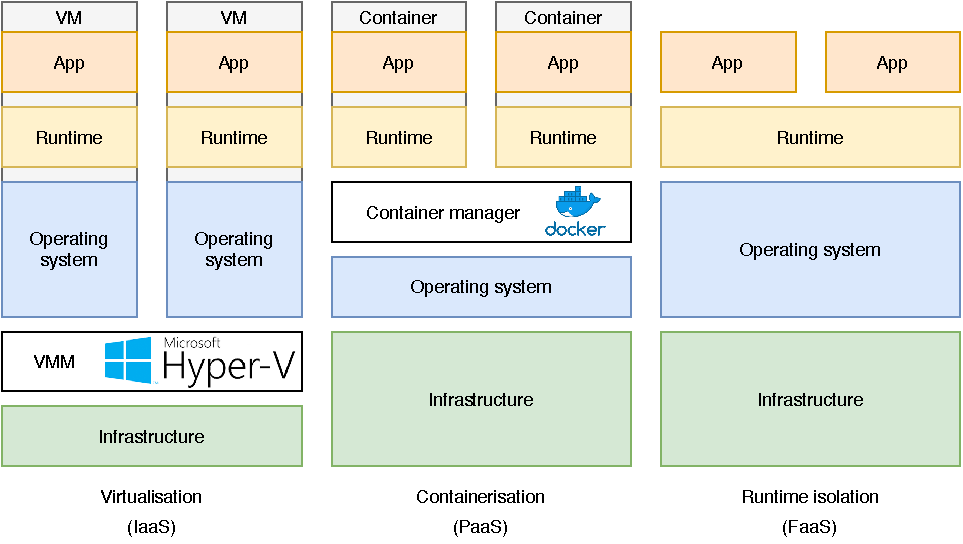
\includegraphics[width=\linewidth]{images/Virt-Cont-Runt.pdf}
    \caption{Different isolation level for an application.}
    \label{fig:virt-cont-runt}
  \end{center}
\end{figure}
\subsection{Virtualisation}
The isolation layer is located either between the hardware and the guest OS (hypervisor of type 1) or between a virtualisation of the hardware, by an hypervisor (type 2) running in another OS, and the guest OS.  In both cases, the guest OS, will run as if it was on a bare-metal machine, executing its own kernel, managing its drivers, its file system, etc.  This is the stronger isolation we can get.  Cloud providers can rent you some Virtual Machines, this is what we call IaaS (Infrastructure as a Service).  You can use many different hypervisor solutions, usually, Cloud providers have their very own solution.
\subsection{Containerisation}
Here we go one level higher, the isolation layer is between the OS and the guest application.  This isolation mechanism is called a container, and is basically a set of processes, running in common namespaces, with a root filesystem different from the host.  Containers share the same kernel as the host though, which means that a process running in a container can be seen from the host.  Containers belong to the world of PaaS (Platform as a Service), a system where Cloud providers offers you to run your application (that you provide under a containerized form) whithout having to worry about all the infrastructure than needs to be deploied along with it, and sometimes even with some great scalability mechanism support.
\subsection{Runtime isolation}
This is the highest level of (weakest) isolation you can get, the isolation is provided by the runtime on which the application is running (ex: The JVM for a Java program, a Python environment, ...).  Multiple guest applications share the same OS, file system, whithout any mechanism to hide it from them.  Cloud providers propose such service under the name of FaaS (Function as a Service).  For this you can provide a small program, that you want to be executed on demand.  Cloud providers usually allocate a container to this program, to provide a safer isolation, but will execute multiple instances of this program in the same containers, to avoid the overhead of creating a new containers each time.  The kinds of programs you usually run in these are computionnaly intensive parts of your application, that needs to have low response time and great scalability (for example resizing of user uploaded images).  This model is often reference as the Lambda model (from Amazon Lambda service) or as serverless computing.

\subsection{INGInious use case}
The case of INGInious is a special one.  The type of the workload caused by the tasks evaluation (fast response time, varying demand, potentially big computation, logic independent of the core application) would suggest to use a serverless strategy, but the isolation requirement are those of PaaS (as the various inputs of the functions are code of student to safely execute, isolated from one another).  And for now the all application relies on IaaS, running in multiple VMs where are hosted the core application and multiple docker agents.  

\section{Containers}
The isolation being the most important requirement, we will then look into containerisation solutions.  Presenting the main concepts behind containerisation, the global container ecosystem, the current solution that INGInious uses and the alternatives we have.

\subsection{Core concepts}
Containers rely on three components: namespaces, control groups and chroot.
\paragraph{}\textbf{Namespaces} are a feature of the Linux kernel since 2002, they are a key element that made containerisation possible.  A namespace can be associated to a context, which is a partition of all the resources of a system that a set of processes has access to, while other processes can't.  Those sets of resources can be of seven kinds:
\begin{itemize}
\renewcommand\labelitemi{--}
  \item \textbf{mnt} (Mount): This controls the mount points.  Processes can only have access to the mount point of their namespace.
  \item \textbf{pid} (Process ID): This allows each process in each namespace to get a process id assigned indepedently of other namespaces porcesses.
  \item \textbf{net} (Network): This provides a virtualized network stack.
  \item \textbf{ipc} (Interprocess Communication): This allows processes of a same namespace to communicate with one another, for example by sharing some memory.
  \item \textbf{uts} (Hostname): This allows to have different hostnames on a same machine, each hostname being considered as unique by the processes of its namespace.
  \item \textbf{user} (User ID): This allows to change the user id in a namespace.
  \item \textbf{cgroup} (Control group): This allows to change the root cgroup directory, this virtualize how process's cgroups are viewed.
\end{itemize}

\paragraph{}When a Linux machine starts, it initiate one namespace of each type in which all the processes run.  The processes can then choose to create and switch of namespaces.

\paragraph{}\textbf{Control groups} are a feature of the Linux kernel that allows to limit and control the resources allocated to some processes.  You can for example control the cpu usage, the memory consumption, the io...  Recently (since kernel 4.5) a new version of cgroups (cgroups v2) appeared, which comes to tackle the flaws of the original implementation, while keeping all of its functionalities.  The main change is the use of a new unified hierarchy to manage the control groups, where all the resources are centralized and where the allocation of some resources is done by adding a sub-resource-group in the hierarchy the current user has access to.
Though, the adoption of the new version is a process, and takes times, and still now many applications use the original version of cgroup (like runc).

\paragraph{}\textbf{Chroot} allows to change the root of the root filesystem for some processes.  For example, we could create a directory \texttt{/tmp/myroot/} which contains all of the usual directories present in the original root folder (\texttt{/}) and set this as the new apparent root for the chosen processes.  This is not a complete sandbox, and not a real isolation on its own, files from outside of the chroot could still be accessed.

\subsection{Storage drivers}
When it comes to handle a container file system, different solutions can be used.  The goal of each is to provide the most efficient writable root directory (\texttt{/}) for each container, but keeping each container inaffected by the modifification done in the other containers.

\paragraph{}In order to do so, three main strategies can be used:
\begin{itemize}
\renewcommand\labelitemi{--}
  \item \textbf{Deep copy}: for each container, the whole image is copied during the creation of the container.  This is simple, but gets terribly slow as the file system size increases.
  \item \textbf{File based copy on write}: for each container, will be copied only the files that are edited during the container life cycle.  This is more complex, but get more efficient as the container's size grows.
  \item \textbf{Block based copy on write}: for each container, will be copied only the blocks (in the filesystem) that are edited during the container life cycle.  This is even more complex, but get more efficient as some small part of big files are edited.
\end{itemize}

\paragraph{}Containers are a specific kind of workload in the sense that many information, data, is redundant in different containers.  For example, for a simple application, we could use several containers with different responsabilities and tools embedded in it, but all based on the same Alpine image.  This brought a new space problem, as we don't want to avoid duplicating too much data.  In order to face this, \textbf{union filesystems} are used, along with layered container images.  This basically means that different container images but with the same basis, will actually share this same basis, avoiding the need to duplicate it.  It differs from file system deduplication mechanism by the level at which the action is taken.  For deduplication, when a block is written on disk, we check if similar data isn't already located somewhere.  Whereas for union file system, the common base image will be read-only, and when an attempt to modify a file is made, a bind mound will be made with a copy of the file on top of the original one, so that the common base stays preserved.

\paragraph{}The storage of a container has to be backed by a file system, which will eventually already provide some interesting mechanisms for the container.  Those four main filesystem used are:
\begin{itemize}
\renewcommand\labelitemi{--}
  \item \textbf{BTRFS}, presented in 2013, \cite{rodeh2013btrfs} is a general purpose file system, based on copy-on-write and with efficient snapshots capabilities and strong data integrity.
  \item \textbf{zFS} is quite similar to BTRFS (but was there before), but handles some mechanisms differently, like the management of blocks (blocks vs. extends\footnote{zFS can have blocks to up to 128KB, while BTRFS will only use the extend strategy (point to the next block).}), snapshots (birth-times vs reference-counting\footnote{When doing snapshots, zFS will store on the block the time at wich a new use of the block has been added, while Btrfs handles it with a reference-counting mechanism.}), ...  It also support deduplication, which can be usefull for system were a lot of data is redundant and disk space is valuable.
  \item \textbf{xFS} is a network file system (as zFS and BTRFS), this means that it can manage several drives in different locations, connected over the network in one storage unit.  It manages to deliver better performances and availability than other similar solutions at the time it was created (1993).\cite{wang1993xfs}  It has no focus on any copy-on-write mechanism as the first two though.
  \item \textbf{ext4} was meant to be the replacement to ext3, as the "Linux Filesystem" when it was presented in 2007. \cite{mathur2007new}  It aims at providing a good balance between scalability, reliability, performance and stability.  It doesn't provide any of the fancy feature of the previous file system.
\end{itemize}

The Table \ref{tab:storage-drivers} present a short summary of the different storage driver available for the different solutions.
\begin{table}[!h]
  \begin{center}
    \begin{tabular}{|l|c|c|c|}
      \hline
      \textbf{Tool} & \textbf{Storage driver} & \textbf{C-o-W}\tablefootnote{Copy-on-write} & \textbf{FS}\tablefootnote{Backing file system}\\
      \hline
      Docker/Podman & \texttt{overlay2} & file based & ext4, xFS \\
      Docker/Podman & \texttt{aufs} & file based & ext4, xFS \\
      Docker/Podman & \texttt{devicemapper} & block based & direct-lvm\tablefootnote{Note that this is a logical volume manager, not a file system, which uses in our case the xFS file system} \\
      Docker/Podman & \texttt{btrfs} & block based & BTRFS\\
      Docker/Podman & \texttt{zfs} & block based & zFS\\
      Docker/Podman & \texttt{vfs} & no & any \\
      \hline
      LXD & \texttt{Btrfs} & block based & BTRFS\\
      LXD & \texttt{ZFS} & block based & zFS\\
      LXD & \texttt{LVM} & yes & ext4\\
      LXD & \texttt{Directory} & no & any \\
      \hline
    \end{tabular}
  \end{center}
  \caption{Summary of storage driver solutions.}
  \label{tab:storage-drivers}
\end{table}

\subsection{Container runtime}
A container runtime is a tool that creates containers, executes process in it, and deletes dead containers.  It will have the responsability to create the namespaces, change the root directory, and attach processes to a control group.  The most common container runtime nowadays is \texttt{runc}, created by the Open Container project.

\subsection{Container manager}
A container manager will use the container runtime, to provide a "user-friendly" interface to manage containers.  It has the responsability to set up the network interfaces, to provide the image of the containers and any Copy-on-write mechanism that could go along with it.  Some of them offer the possibility to create custom images, to create pods, or swarm, which are entities of multiple interconnected containers.

\subsection{Rootless containers}
As we saw previously, creating a container requires to create a bunch of namespaces, and launch some processes in it, limiting their resources with control groups.  If you don't do this manually, all of this is taken care of by the container runtime.  There are two modes in which you can run containers:
\begin{description}
  \item[Rootfull]  This is the default choice when using Docker, the processes launched in the container are owned by root, and the container runtime is executed as root as well.  The container manager also need root permissions then.  It means that either the user willing to launch a container has to be root, or some trick has to be used to allow the user to gain the priviledge required to launch the containers.  Docker does it by allowing any user member of the group \texttt{docker} to send requests to the daemon, which runs as root and can do the required operations.
  \item[Rootless] This is less common, and much more secure.  The processes launched in the container are not owned by root (but are mapped to the root uid inside the container) and the container runtime is not executed as root either.  This requires the use of second generation control group to have resource management capabilities, as the unified hierarchy allows any user to create more sub-resource-group, to manage the resource it has access to.  It means that we don't need to use a daemon or any other trick to give a user permission to do "root stuff" on the host.
\end{description}
There is also an intermediate solution, which actually map the root user of the container to an unpriviledged user on the host, as in the rootless case.  It means that processes running as root in the container won't be root on the host, which is already better, but the container runtime still runs as root.

\section{Ecosystem overview}
A small overview of the current container ecosystem can be found on Figure \ref{fig:overview}.  Note that solutions like Kubernetes\footnote{Kubernetes is "an open-source system for automating deployment, scaling, and management of containerized applications" \cite{kubernetes}} which are more oriented towards hosting and continuous deployment of container based applications than to single container provisionning are not presented here\footnote{A more detailed overview dor those kind of applications is provided by Containerd at the following address: \href{https://containerd.io/img/architecture.png}{https://containerd.io/img/architecture.png}}.
\begin{figure}[h!]
  \begin{center}
    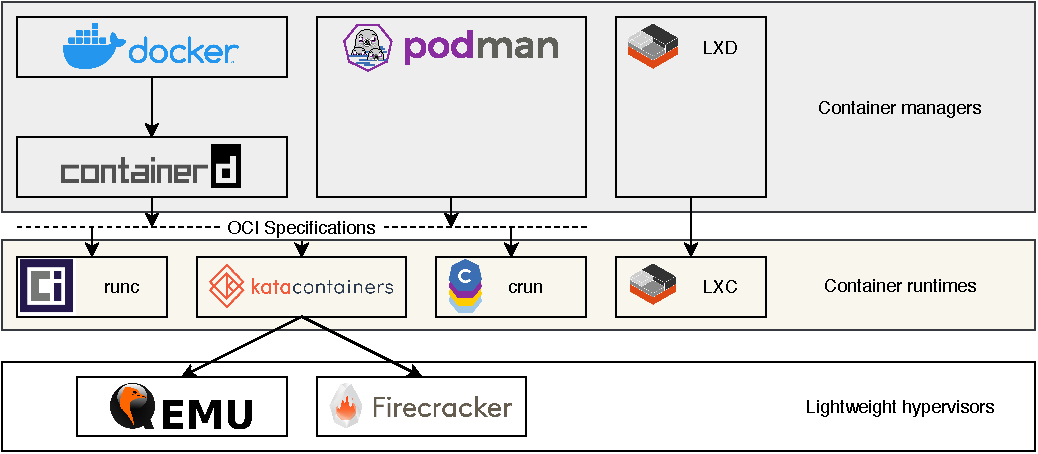
\includegraphics[width=\linewidth]{images/ecosystem.pdf}
    \caption{Small overview of the current container ecosystem}
    \label{fig:overview}
  \end{center}
\end{figure}
\paragraph{}\textbf{OCI} (Open Container Initiative) is "an open governance structure for the express purpose of creating open industry standards around container formats and runtime."\cite{oci} They currently have two specifications: the format of the image that has to be given to an OCI compatible runtime, and the commands to interact with such runtime.

\section{Containerisation solutions}
\paragraph{}\textbf{Docker}\cite{merkel2014docker} is today probably the most known solution for containerization.  Since its apparition in 2014, its interest for the PaaS sector hasn't ceased to grow.  It consists in a daemon, running on the host, that allows to easily manage different containers.  It relies on Containerd, "An industry-standard container runtime with an emphasis on simplicity, robustness and portability"\cite{containerd}, which is a more complete container runtime than what I presented before, with embedded network management, storage driver management, and other mechanism.  Containerd is not meant to be used standalone though, which is why we still use Docker.  By default, Docker uses \texttt{runc} as container runtime by default, but is compatible with any runtime that fulfill the OCI\cite{oci} requirements.

The main advantages of Docker are its simplicity of use, its production-grade quality, the huge fleet of ready-to-run containers publicly available and a lot of useful tools (like \texttt{docker-swarm} that come along with it).  This is the solution currently used by INGInious.

\paragraph{}"\textbf{Podman} is a daemonless container engine for developing, managing, and running OCI\cite{oci} Containers on your Linux System."\cite{podman}  Podman presents itself as a viable true alternative to Docker.  Its main difference is the fact that it runs daemonless, it runs containers as detached child processes and containers can be rootless by default (while it is only a recent feature coming up to Docker).  It can also manage pods, which are groups of containers deployed on the same machine. Its default runtime is \texttt{runc} as well.  Podman is an Open-Source project, and is still growing a lot, the latest version at this day (2020-02-28) is v1.8.0, released 21 days ago, and already 287 commits have been done since then!

\paragraph{}"\textbf{LXC} is a userspace interface for the Linux kernel containment features."\cite{lxc}  This solution is developed and maintained by Canonial Ltd.  Docker used to be based on LXC until it created its own execution environment.  LXC came out recently with a new solution; LXD, which offer about the same things as Docker does.  A bunch of ready to run images publicly available, and a nice command line interface to interact with containers.  The only missing feature of LXD compare to Docker, regadering our use case, is the possibility to launch a container with a command, and stop it when it is finished.  LXC actually start a complete init process for each container, in which you can then come and execute your command.

\paragraph{}\textbf{Linux-VServer}\cite{linux-vserver} is a bit of a special one.  No namespaces are used to provide isolation here, they rely on contexts to separate multiple virtualised systems.  They have modified the Linux kernel to provide some utilities like process isolation, network isolation and CPU isolation.  The main advantage of this approach is scalabality as it can run a large amount of containers, the drawback is the portability.  It requires a modifed version of the kernel and it also misses some features like checkpoint and resume that we can have with more classical containerization and real virtualisation.  This is an project much older than Docker and its contemporaries and differ in goal, it is not appropriate for the INGInious workload.  This is an experience more similar to what classical VM provides, where you will setup multiple application in one environnment.  The container is not build for one single purpose.

\paragraph{}\textbf{OpenVZ}\cite{openvz} is another container-based virtualisation solution.  But this time they use namespaces to provide it.  They also have their own way of dealing with system resources management, more complete than cgroup.  Even though this is more close to what runc and LXC provide in therm of isolation, this is still not the kind of experience appropriate for INGInious use case.  This is designed, as for Linux-VServer, for a more complete server experience.

\paragraph{}\textbf{Kata Containers} is not another container manager.  It is an OCI compatible runtime.  With the specificity that it doesn't run mainstream containers as \texttt{runc}, but actually lightweight virtual machines, using KVM virtualisation and with Qemu (originally), Firecracker or Cloud Hypervisor (still in its early days) as hypervisor.  Those two first currently available hypervisor are not really equivalent though, as the original one has more features (like devices assignment) and the second one has lower memory footprint, smaller attack surface (smaller code base), and a shorter boot time.
They put forward four features of their solution:
\begin{itemize}
\renewcommand\labelitemi{--}
  \item \textbf{Security}: Thanks to their virtualization solution, each runtime has its own kernel, with real network, i/o and memory isolation.
  \item \textbf{Compatibility}:  They support industry standarts, as the OCI\cite{oci} and legacy virtualization technologies.
  \item \textbf{Performance}:  Their performances are consistent with classical containerization solutions.
  \item \textbf{Simplicity}:  They eliminate the need to have a virtual machine dedicated to host containers.
\end{itemize}

\paragraph{}\textbf{crun} is a complete equivalent of \texttt{runc}, yet another OCI compatible runtime, but this one is implemented in C, which give it a small performance advantage over \texttt{runc}, implemented in GO.  \texttt{crun} has also full support for cgroupv2, which is still lacking for \texttt{runc} at the moment (2020-04-22).

  \chapter{Related work}

In this chapter I will present some of the work that has already been done in the field of containerization, and show what we can take from it.  I will then explain why my work adds up something to those previous research.

\section{Container and Virtual Machine performances}
As said previously, Virtual Machines have been kept away from the PaaS world, because of the greater overhead that Virtualization has on booting time and resources consumptions of the isolated system created.  This paper \cite{dua2014virtualization} made a detailed point about it back in 2014, emphasizing on three points that needed to be improved for the next generation of containers: Security, OS Independence and Standardization.  The last one meaning that containers runtime should establish some common requirements, come up with a common container format.  We have seen this appear since then, under the OCI (Open Container Initiative) specifications.  A thradeoff with the performances (mostly I/O) of the application running isolated is much more evident with virtualisation than with containerisation\cite{felter2015updated}.

\paragraph{}But recently things started to change, some new solutions seem to have the advantage of both sides, the isolation of a VM and the portability and lightness of a Container.  This is why some VM-based solution are presented here.  Even though VMs do not come from the same domain of application as Containers, and even though in the case of INGInious, Containers were 5 years ago the obvious choice, it might now be time to reconsider it.

\section{SAND} 
\paragraph{}SAND\cite{akkus2018sand} aims at improving the performance of serverless computing with two techniques: application-level sandboxing, and a hierarchical message bus:
\begin{itemize}
\renewcommand\labelitemi{--}
  \item \textbf{Application Sandboxing}: The key idea here is to differentiate multiple executions of different functions with multiple execution of a same function.  In the first case, as usual, a new container is launched on the new function demand and the function is executed inside of it.  In the second case, instead of lauching a new container with exactly the same configuration as an already running one, we only fork a process inside de running container to deal with the new demand, which is much faster than creating a new container.  The problem in our case, is that we loose the isolation between student code execution, which is not desirable.
  \item \textbf{Hierarchical Message Queuing}: The goal to this is to facilitate communication between functions that interact with one another (i.e. the output of a function is the input of another one).  To do so they use a two-level communication bus: global and local.  Global means that the communication is made between different functions on different hosts, while local means different functions on the same host.  As accessing the local bus is much faster than the global one, it can decrease latency for functions on the same host.  % In our case, as INGInious is still running on a single host, this shouldn't improve our performances that much.  But in a near future where INGInious get a new horizaontally scaled architecture, it might be interesting to come back on it.
\end{itemize}

\section{SOCK} \label{subsec-sock}
\paragraph{}"Sock (roughly for serverless-optimized containers), [is] a special-purpose container system with two goals: (1) \textit{low-latency invocation} for Python handlers that import librairies and (2) \textit{efficient sandbox initialization} so that individual workers can achive high ready-state throughput." \cite{oakes2018sock}  The final product created here isn't really something we could use for INGInious, it is a serverless solution (based on the Lambda model), targeting specifically python applications.  Though, in the process of creating this solution, they started from containers and deconstructed their perfromances, indentifying their bottlenecks.  And from this we can take those things:
\begin{itemize}
\renewcommand\labelitemi{--}
  \item Bind mounting is twice as fast as AUFS.  Even though AUFS (used by Docker) as a usefull Copy-on-write capability, we don't need to write to most of our files in our case, so using a read-only bind mounting for those files could allow us to avoid copying all file before startup, while still beeing able to edit the one with want to.
  \item Network namespaces creation and cleanup are costly, due to a single lock shared across all network namespaces.  We might gain some performances buy not adding network interfaces to containers that don't need it.
  \item Reusing a cgroup is at least twice as fast as creating a new one each time.  We could keep a pool of initialized cgroups, and only change the current container it controls.
\end{itemize}

\section{LightVM} 
\paragraph{}LigthVM is a complete redesign of Xen's toolstack which tried to bring some container's characteristics to VMs.  Such as fast instantiation (small startup time) and high instance density capability (high number of instances running in parallel on the same machine).\cite{manco2017my}  Xen is a Type-1\footnote{A Type-1 hypervisor is an hypervisor that runs on a bare-metal machine, whithout additional host.} hypervisor presented in 2003 with really low virtualization overheads and high hosting capacity, allowing a machine to host up to a 100 guest OS.\cite{barham2003xen}  
\paragraph{}They achieve such container's like performances by:
\begin{itemize}
\renewcommand\labelitemi{--}
  \item reducing the image size and the memory footprint of virtual machines.  They do so by including in the VM only what is necessary to the application that is meant to be executed in it.
  \item introducing noxs (no XenStore), a new implementation of Xen, without XenStore (which was a real bottleneck for fast instantiation of multiple VMs).
  \item splitting the Xen's toolstack into what can be run before the VM creation and what as to be done during it.  Allowing to pre-initialize VMs.
  \item replacing the Hotplug Script by xendevd, a binary deamon that can execute pre-defined setup more efficiently.
\end{itemize}

\paragraph{}They present four use cases with this solution, one of them beeing more intreresting for us: lightweight computation services, for which they rely on Minipython unikernel, to run computations written in Python, as a Faas could propose to do.  This would still be hard to use for INGInious, for the same reason as for SOCK (§\ref{subsec-sock}).

\section{Firecracker} 
\paragraph{} Firecracker is a new VMM (hypervisor) created specifically for serverless and containers applications.  \cite{agachefirecracker}  This is a solution provided by AWS, that very recently got deployed for two of their web services: Lambda (Faas) and Fargate (Paas).  We are basically getting here the good isolation of virtual machines and nearly as good performances and low overhead of containers.  Firecracker is based on KVM and provides minimal virtual machines (MicroVMs).  The configuration is done through a REST API.  Device emulation is available for disks, networking and serial console.  Network can be limited and so can disk throughput and request rate.  If proven to be easily usable in INGInious case, this would provide a better alternative to Docker regarding security.

\section{Summary}
\paragraph{}In this section, on Table \ref{tab:summary}, are quickly reminded the several solutions we explored in this chapter, along with some interesting infos about them.
\begin{table}[!h]

  \begin{center}
    \begin{tabular}{|p{.2\textwidth}|p{.1\textwidth}|p{.1\textwidth}|p{.1\textwidth}|p{.1\textwidth}|p{.1\textwidth}|p{.1\textwidth}|}
       \hline
       \textbf{Name} & \textbf{Pub.} & \textbf{Update} & \textbf{Open-Source} & \textbf{Pot. Sol.} & \textbf{Com.} & \textbf{Isol.} \\
       \hline
       SAND & 2018 & ? & ? & No & No & Cont. \\
       \hline
       SOCK & 2018 & ? & ? & No & No & Cont. or Runt. \\
       \hline
       LigthVM & 2017 & 2017 & Yes & No & No & Virt. \\
       \hline
       Firecracker & 2019 & 2020 & Yes & Yes & Yes & Virt.\\
       \hline
    \end{tabular}
  \end{center}
  \caption{Summary table of the different solutions explored in this chapter.}
  \label{tab:summary}
\end{table}
\paragraph{}\textbf{Caption}: 
\begin{itemize}
  \item \textit{Name}: The name of the project.
  \item \textit{Pub.}: The first publication year of the project.
  \item \textit{Update}: The last update year of the project.
  \item \textit{Open-source}: If the project is open-source.
  \item \textit{Pot. Sol.}: If the project could be a solution in our case.
  \item \textit{Com.}: If the project is a "commercial grade" solution.
  \item \textit{Isol.}: The type of isolation used in the project.
  \item \textit{Cont.}: Isolation by containerization.
  \item \textit{Virt.}: Isolation by virtualization.
  \item \textit{Runt.}: Isolation by the runtime of the application.
\end{itemize}

\section{My master thesis}

  \chapter{Testing}

As previously said, the goal of this thesis will be to identify if some improvements could be made to INGInious, by changing the containerization solution in use.  To do this, I have created some tests and listed different possible configurations that should face those tests.  Based on the results of those tests, I should be able to determine whether or not we can bring improvement to INGInious.

\section{Setup}
\subsection{Testing environment}
To be fair in the result comparison, all the different configurations have to be tested with as much in common as possible.  This will allow us to determine the influence of varying parameters in those configurations.  To do so, the same machine will be used for all the tests, with its configuration being updated accordingly to the requirements of each solution.

The testing environment used for the final results presented in this work is an old laptop, refurbished with the following configuration:\\
\begin{tabular}{rl}

  \textbf{processor} & Intel(R) Core(TM) i5-2410M CPU @ 2.30GHz (x4) \\
  \textbf{memory} & 8GB \\
  \textbf{storage} & 256GB SSD \\
  \textbf{operation system} & Ubuntu 18.04.4 LTS \\
  \textbf{linux kernel version} & 4.15.0-101-generic \\

\end{tabular}


The choice of going with a bare-metal setup was not the original one.  But the early results I got showed that some solutions (especially the ones using virtualization) did perform way worse when running inside of a VM.  To get the best out of them, the setup has then been moved out of VMs.

\paragraph{}\textbf{Note about cpu:}  The cpu is a little bit weak, and not representative of what a real production server would use to host a container workload.  Unfortunately, this was all I had available, and it will have to do.  This means that the results presented in this work can still be a little bit less performant than what we could get typically in the cloud.
\paragraph{}\textbf{Note about memory:}  This is also typically less than what we would have in the cloud, but this is just enough for our case, as we only execute one container at a time, with limited access to memory.
\paragraph{}\textbf{Note about storage:}  The storage type is important, as it will highly influence the performance of my tests, given the high solicitation of I/O they require.  Using an SSD is therefore essential, both to avoid the need to run the tests for several weeks, and to have measurements more in pair with what cloud provider proposes.
\paragraph{}\textbf{Note about operating system:}  The main reason I have chosen Ubuntu is that I am familiar with it, and it made things easier for me to set up.  Also, Ubuntu is often (if not always) an option that cloud providers offer when it comes to choosing the OS to install in a VM.

\subsection{Configuration of the environment}
As a lot of different solutions are going to be tested, and all of them with their requirements (sometimes conflicting with the ones of other solutions), some work had to be done to make it easier for someone to replicate them.  The configuration of the environment is done with Ansible\footnote{https://docs.ansible.com/} playbooks, with one playbook for each solution to test.

All the different configurations are presented in section \ref{subs:candidates}.  The different playbooks can be found in the repository of this project at this address: \href{https://github.com/edvgui/LEPL2990-Benchmark-tool/tree/master/ops}{https://github.com/edvgui/LEPL2990-Benchmark-tool/tree/master/ops}. 

\section{Tests}
As we already said previously, time is an important aspect of the experience INGInious provides to its users.  The time for a task to be evaluated and the time before this task is evaluated.  To improve those two, in those tests we will focus on the booting time of containers and their IO handling (still related to the time overhead that some solution could have compared to another).

While we are at it, we will also verify if some solutions handle network much poorly than others.  Each test is presented in more detail in section \ref{subs:experiments}.


\subsection{Candidates}\label{subs:candidates}
A candidate solution is a combinaison of different elements, variabilities, choices to make.  We will consider here those ones:
\begin{itemize}
  \renewcommand\labelitemi{--}
  \item \textbf{Container manager}: \textit{Docker}, \textit{Podman}, \textit{LXD}, those are the different user friendly solution that can be used to manage container, and that we will compare here.
  \item \textbf{Container runtime}: \textit{runc}, \textit{crun}, \textit{LXC}, \textit{Kata containers} (Qemu or Firecracker), the (less user-friendly) container runtimes, taking care of all the isolation that a container require.
  \item \textbf{Control group}: \textit{cgroup} and \textit{cgroupv2}, there is no real choice to make here: cgroupv2 is the successor of cgroup, and should be used, when supported by the other elements of the configuration.
  \item \textbf{Storage driver}: \textit{aufs}, \textit{btrfs}, \textit{devicemapper}, \textit{directory}, \textit{overlay}, \textit{vfs}, \textit{zfs}, \textit{lvm}, those are the different strategies that can be used to manage the file system of the container.
  \item \textbf{Base container image}: \textit{Alpine} because it is the default choice when it comes to conceive containerized applications today or \textit{Centos} because it is the current choice made by INGInious.
  \item \textbf{Rootless container}: Whether if we run the container in rootless mode.
\end{itemize}

Though, we cannot compose a candidate solution with one element of each category, randomly picked.  Some elements of the solution might only be usable with some of the possibilities for a variability.  The different constraints that we have are listed here:
\begin{itemize}
  \renewcommand\labelitemi{--}
  \item Docker does not support cgroupv2 yet (actually the support has to be added by containerd).
  \item Docker only supports aufs (deprecated), btrfs, devicemapper (until Docker 18.06), overlay, vfs, zfs as storage driver.
  \item LXD does not support cgroupv2 yet.
  \item LXD only supports LXC as runtime, and LXC is only supported by LXD.
  \item LXD only supports btrfs, zfs, directory (dir) and lvm as storage driver.
  \item Kata Container with Firecracker only supports devicemapper as a storage driver.
  \item zfs, lvm, aufs cannot be used with rootless containers.
  \item cgroup (v1) cannot be used with rootless containers.
  \item runc does not support cgroupv2 yet.
  % TODO Check if kata-runtime is compatible with cgroupv2
\end{itemize}

The list of different candidate solutions we can compare is presented in the table below.  Each container will be launched with a CPU limitation of one single-core, and memory limitation of 1GB.  This is more than enough for each test that will be done.  A network interface will be only added to the container if it needs it for the specific test.\\\\

\newcounter{rowno}
\setcounter{rowno}{0}
\begin{longtable}{|>{\stepcounter{rowno}\therowno}r|c|c|c|c|c|c|}
  \hline
  \multicolumn{1}{|r|}{\#} & \textbf{Manager} & \textbf{Image} & \textbf{Storage} & \textbf{Cgroup} & \textbf{Runtime} & \textbf{Rootless} \\ \hline \hline
   & Docker & Alpine & aufs          & v1 & runc       & No\\ \hline
   & Docker & Alpine & btrfs         & v1 & runc       & No\\ \hline
   & Docker & Alpine & devicemapper  & v1 & runc       & No\\ \hline
   & Docker & Alpine & overlay2      & v1 & runc       & No\\ \hline
   & Docker & Alpine & vfs           & v1 & runc       & No\\ \hline
   & Docker & Alpine & zfs           & v1 & runc       & No\\ \hline
   & Docker & Alpine & aufs          & v1 & crun       & No\\ \hline
   & Docker & Alpine & btrfs         & v1 & crun       & No\\ \hline
   & Docker & Alpine & devicemapper  & v1 & crun       & No\\ \hline
   & Docker & Alpine & overlay2      & v1 & crun       & No\\ \hline
   & Docker & Alpine & vfs           & v1 & crun       & No\\ \hline
   & Docker & Alpine & zfs           & v1 & crun       & No\\ \hline
   & Docker & Alpine & aufs          & v1 & kata-runtime\footnote{Default Kata Containers runtime, using qemu as hypervisor.}  & No\\ \hline
   & Docker & Alpine & btrfs         & v1 & kata-runtime  & No\\ \hline
   & Docker & Alpine & devicemapper  & v1 & kata-runtime  & No\\ \hline
   & Docker & Alpine & overlay2      & v1 & kata-runtime  & No\\ \hline
   & Docker & Alpine & vfs           & v1 & kata-runtime  & No\\ \hline
   & Docker & Alpine & zfs           & v1 & kata-runtime  & No\\ \hline
   & Docker & Alpine & devicemapper  & v1 & kata-fc\footnote{Kata Containers runtime, using Firecracker as hypervisor}    & No\\ \hline
   & Docker & Centos & aufs          & v1 & runc       & No\\ \hline
   & Docker & Centos & btrfs         & v1 & runc       & No\\ \hline
   & Docker & Centos & devicemapper  & v1 & runc       & No\\ \hline
   & Docker & Centos & overlay2      & v1 & runc       & No\\ \hline
   & Docker & Centos & vfs           & v1 & runc       & No\\ \hline
   & Docker & Centos & zfs           & v1 & runc       & No\\ \hline
   & Docker & Centos & aufs          & v1 & crun       & No\\ \hline
   & Docker & Centos & btrfs         & v1 & crun       & No\\ \hline
   & Docker & Centos & devicemapper  & v1 & crun       & No\\ \hline
   & Docker & Centos & overlay2      & v1 & crun       & No\\ \hline
   & Docker & Centos & vfs           & v1 & crun       & No\\ \hline
   & Docker & Centos & zfs           & v1 & crun       & No\\ \hline
   & Docker & Centos & aufs          & v1 & kata-runtime  & No\\ \hline
   & Docker & Centos & btrfs         & v1 & kata-runtime  & No\\ \hline
   & Docker & Centos & devicemapper  & v1 & kata-runtime  & No\\ \hline
   & Docker & Centos & overlay2      & v1 & kata-runtime  & No\\ \hline
   & Docker & Centos & vfs           & v1 & kata-runtime  & No\\ \hline
   & Docker & Centos & zfs           & v1 & kata-runtime  & No\\ \hline
   & Docker & Centos & devicemapper  & v1 & kata-fc    & No\\ \hline
   & LXD    & Alpine & btrfs         & v1 & LXC        & No\\ \hline
   & LXD    & Alpine & zfs           & v1 & LXC        & No\\ \hline
   & LXD    & Alpine & directory     & v1 & LXC        & No\\ \hline
   & LXD    & Alpine & lvm           & v1 & LXC        & No\\ \hline
   & LXD    & Centos & btrfs         & v1 & LXC        & No\\ \hline
   & LXD    & Centos & zfs           & v1 & LXC        & No\\ \hline
   & LXD    & Centos & directory     & v1 & LXC        & No\\ \hline
   & LXD    & Centos & lvm           & v1 & LXC        & No\\ \hline
   & Podman & Alpine & aufs          & v1 & runc       & No\\ \hline
   & Podman & Alpine & btrfs         & v1 & runc       & No\\ \hline
   & Podman & Alpine & overlay       & v1 & runc       & No\\ \hline
   & Podman & Alpine & vfs           & v1 & runc       & No\\ \hline
   & Podman & Alpine & zfs           & v1 & runc       & No\\ \hline
   & Podman & Alpine & aufs          & v2 & crun       & No\\ \hline
   & Podman & Alpine & btrfs         & v2 & crun       & No\\ \hline
   & Podman & Alpine & overlay       & v2 & crun       & No\\ \hline
   & Podman & Alpine & vfs           & v2 & crun       & No\\ \hline
   & Podman & Alpine & zfs           & v2 & crun       & No\\ \hline
   & Podman & Alpine & btrfs         & v2 & crun       & Yes\\ \hline
   & Podman & Alpine & overlay       & v2 & crun       & Yes\\ \hline
   & Podman & Alpine & vfs           & v2 & crun       & Yes\\ \hline
   & Podman & Centos & aufs          & v1 & runc       & No\\ \hline
   & Podman & Centos & btrfs         & v1 & runc       & No\\ \hline
   & Podman & Centos & overlay       & v1 & runc       & No\\ \hline
   & Podman & Centos & vfs           & v1 & runc       & No\\ \hline
   & Podman & Centos & zfs           & v1 & runc       & No\\ \hline
   & Podman & Centos & aufs          & v2 & crun       & No\\ \hline
   & Podman & Centos & btrfs         & v2 & crun       & No\\ \hline
   & Podman & Centos & overlay       & v2 & crun       & No\\ \hline
   & Podman & Centos & vfs           & v2 & crun       & No\\ \hline
   & Podman & Centos & zfs           & v2 & crun       & No\\ \hline
   & Podman & Centos & btrfs         & v2 & crun       & Yes\\ \hline
   & Podman & Centos & overlay       & v2 & crun       & Yes\\ \hline
   & Podman & Centos & vfs           & v2 & crun       & Yes\\ \hline
\end{longtable}

\subsection{Experiments} \label{subs:experiments}
For all the experiments presented here, time measurements are taken at four important steps of the execution of the container:
\begin{description}
  \item[$t_0$] Before its creation, this is time zero.
  \item[$t_c$] After its creation. Container's state is \textit{created}.
  \item[$t_s$] After its startup. Container's state is \textit{running}.
  \item[$t_e$] After the end of the execution of the command. Container's state is \textit{running}.
\end{description}
This gives us three interesting measurements:
\begin{enumerate}
  \item Creation time: $t_{create}=t_c - t_0$
  \item Starting time: $t_{start}=t_s - t_c$
  \item Execution time: $t_{exec}=t_e - t_s$
\end{enumerate}

The command available to interact with each step of the lifecycle of the containers for each solution can be found in Appendix \ref{appendix:container-life-cycle}, along with some more explanation about what is done in each step.

To do this, each container will be running as first process a shell\footnote{except for LXD, which natively has an init process running in each container}, which will never receive any input, but is here to ensure that the container will stay up as long as we need it.  When we do not need the container anymore, we simply kill all the processes in it.

\subsubsection{Booting time}
This test aims at determining the candidate solution that can provide a ready to run container the fastest.  To measure this, a simple container composed of only the base image is created, in which the simple command \texttt{/bin/echo Hello World} is executed.  The best candidate would be the one that has the shortest creation and starting time ($t_{create} + t_{start}$).  The execution time ($t_{exec}$) is also a good illustration of the overhead caused by all the steps taken before actually starting the process in the container.

\subsubsection{Basic I/O performances}
Those tests aim at determining mostly the influence of the usage of each storage driver on the performances of an application that relies highly on it.  Four different tests are done here: big file read and write, and a great amount of file read and write.  The best candidate solution would be the one with the shortest creation, starting and execution time ($t_{create} + t_{start} + t_{exec}$).

For the first one, five SQLite databases have been created, of five different size (\texttt{151.6 kB}, \texttt{536.6 kB}, \texttt{2.6 MB}, \texttt{11.9 MB} and \texttt{111.6 MB}, about one order of magnitude apart from each other).  We use an SQLite database as everything will be stored in one file, and no daemon needs to be running, which simplifies the setup of the tests.  Plus this is a more realistic workload than just reading/writing one gigantic file.
The reading test will do a select operation on each table of the database without any filter, displaying all of the table content.  The writing test will duplicate each table in the database.  The database chosen as basis to generate all the presented one is \texttt{tpcc}\footnote{\href{https://relational.fit.cvut.cz/dataset/TPCC}{ttps://relational.fit.cvut.cz/dataset/TPCC}}, which is a benchmark database, perfect for our case.  The biggest database used is an export from the tpcc database, the other ones are created by removing the content of some tables from this same database.

For the second one, five loads of small file have been created (10, 100, 1000, 10 000 and 100 000 files).  The content of the file is alphanumeric and completely random (no file should be a duplication of another one), each file is $4096$ character (and bytes) long.  This represents the best the usual kind of file a user could access, to read or write content from/to it. 
The reading test will load the content of each file in memory, then discard it and move to the next one.  The writing test will extract an uncompressed archive (\texttt{tar}) containing all those files.

\subsubsection{Network setup time}
This test aims also at determining the candidate solution that can set up a ready to run container the fastest, but with the increased complexity of adding a network interface, and mapped ports, so that the host machine can send requests to an HTTP server running inside of the container.  I have chosen a \texttt{lighttpd} server, for its lightness, and its wide use in container application.  It takes one more time measurement here, the time at which we received the first response at the HTTP requests we send to our server ($t_r$).  The best candidate would be the one that has the shortest delay before this response ($t_{create} + t_{start} + t_{exec} + t_{response}$, with $t_{response}=t_r - t_e$).  The execution time corresponds to the execution of the command that launches the server as a detached process.

\subsubsection{Ping response time}
This really simple test aims at determining if some solution provides a much weaker network solution to the container than the others.  We simply perform a ping request to \texttt{1.1.1.1}, and compare the response time we get for each solution.  The best solution would be the one with the shortest ping response time.

  \chapter{Results interpretation}

Based on the results of the different experiments I made, I will try to answer in this chapter to three main questions:
\begin{enumerate}
  \item Compared to other available solutions, how good is the current configuration chosen by INGInious to face the responsiveness challenge of the platform?  How much better could it be?  How easy would it be to improve it?
  \item Could there be a solution tailor-made for the specific case of INGInious?  What would it be?  What would it cost to use it?
  \item What would be the cost of providing a stronger/safer isolation to the containers used by INGInious?  What opportunities could it bring?
\end{enumerate}

\section{Current INGInious situation}
We will here consider the first question:
\begin{center}
  \say{\textit{Compared to other available solutions, how good is the current configuration chosen by INGInious to face the responsiveness challenge of the platform?  How much better could it be?  How easy would it be to improve it?}}
\end{center}

The current configuration of INGInious is the following:
\begin{center}
\begin{tabular}{rl}
  \textbf{Container manager} & Docker \\
  \textbf{Base image} & Centos \\
  \textbf{Storage driver} & overlay2 \\
  \textbf{Container runtime} & runc \\
  \textbf{Control group version} & v1 \\
  \textbf{Rootless containers} & no \\
\end{tabular}
\end{center}

This configuration is quite decent, and gives good performances, their is mainly one change that can improve those.  But let's analyse this step by step.

\subsubsection{Storage driver}
Overlay2 (referenced for the rest of this discussion as simply overlay) is the storage driver that Docker recommands to use by default (when OverlayFS is supported on the host).  Its layer mechanism allows to limit the redundancy of information when you use the same base image to create different images.  And its file-based copy-on-write strategy gives overal good performances.

\begin{figure}[h!]
  \begin{center}
    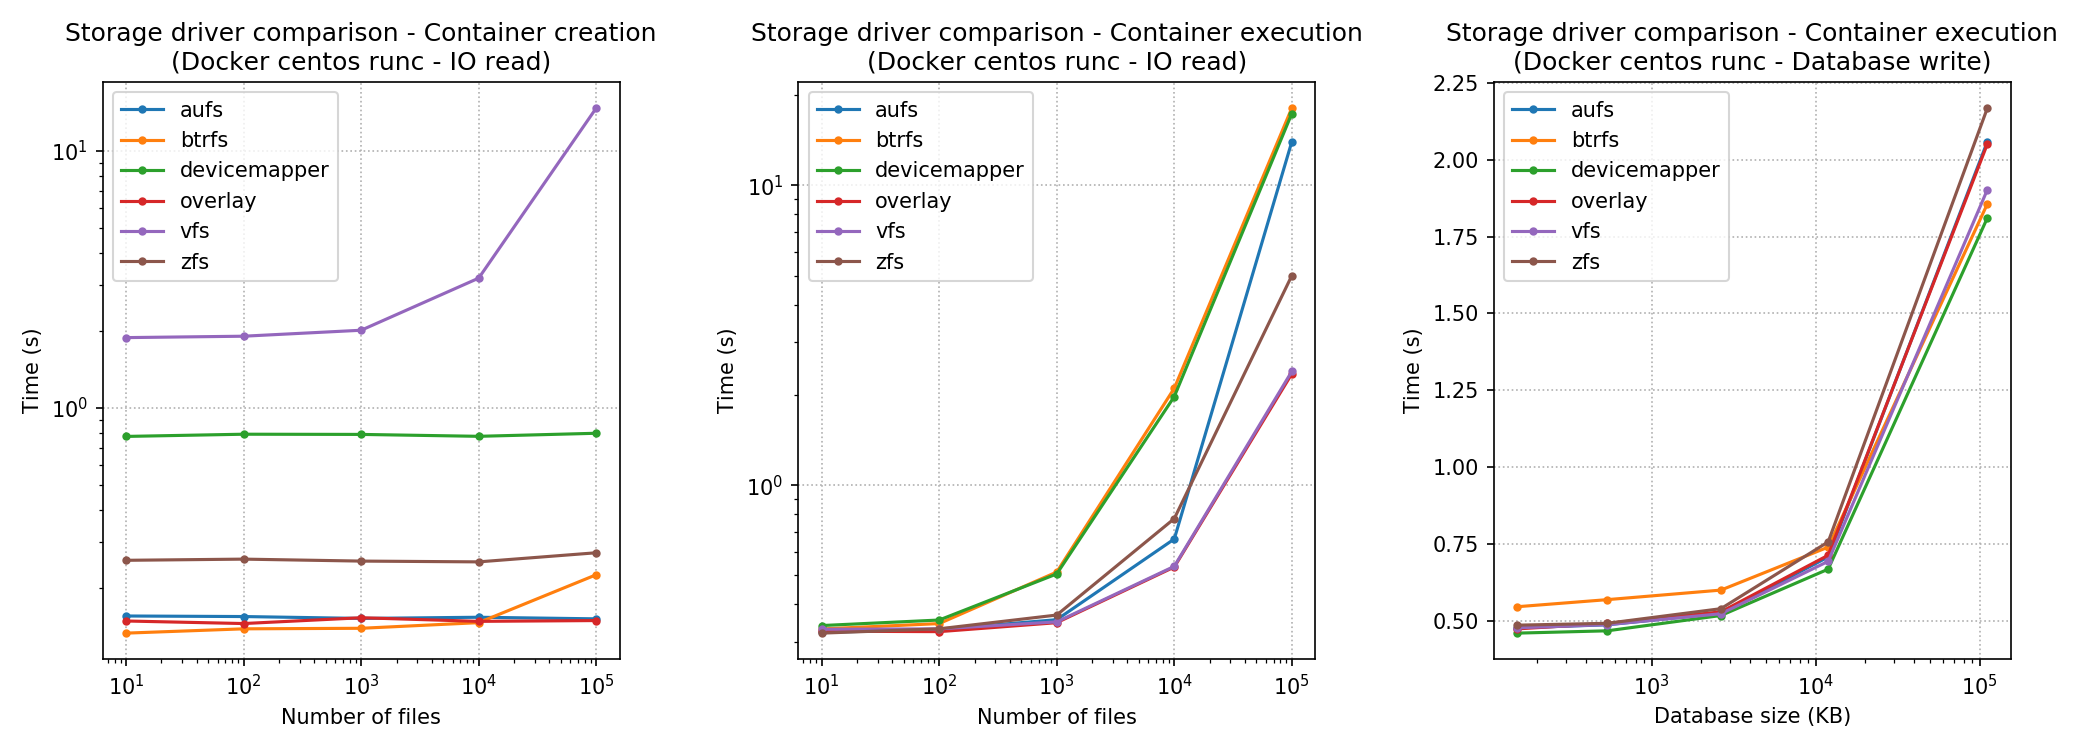
\includegraphics[width=\linewidth]{images/question-1-storage-driver.png}
    \caption{Storage driver performance comparison for Centos containers, launched with Docker and runc}
    \label{fig:q1:storage-driver}
  \end{center}
\end{figure}

On Figure \ref{fig:q1:storage-driver}, we can see how much it cost to have a full-copy mechanism like vfs for each container creation.  We can also see that overlay, aufs and btrfs offers similar performances for the creation of containers.  The main differences between those three is shown by their performance when solicitating I/O.  
\begin{itemize}
  \item Aufs, even though performing similarly to overlay in all the other cases (not shown here) and relying on the same union file system mechanism as overlay, gets far behind the latest when a lot of read operations are done.  This most likely comes from one big difference in the implementation of those two union file system: when a file is opened with OverlayFS, all the operations on it are directly managed by the underlying file systems.  This simplify the implementation, and improve the performances quite a lot as we can see on the second graph of the figure.  (For this test, for each \texttt{openat} system call, four \texttt{read} system call are done)
  \item On the last graph of the figure (on the right), we can see the advantage of using block-based copy-on-write, when modifying big files.  Indeed, when doing so, where overlay and aufs will need to copy the whole file before modifying it, the other solutions will only need to copy the file system blocks needing to be modified (or not even copy the file in the case of vfs).  We can see that devicemapper handles this a little bit better than btrfs, but given the much higher container creation cost of the first one, it will most likely be more intersting to use btrfs in most cases.
  \item One more thing to pay attention to, is that is seems that storage drivers with block-based copy-on-write mechanism, face some difficutlies when creating container with a large amount of files in it.  This might be harder to see here for devicemapper and zfs, but it is the case.  Zfs seems to also suffer from big files in the container filesystem, for the container creation.
\end{itemize}
One more reason to justify the use of overlay is that in most container use cases, read operations are the most important ones.  Normally, no large amount of data should be written in the container file systems, volumes (external storage from the host, mounted into the container file system) should specifically be used for that purpose as it provide nearly native writing performances and the data persists, even after the end of the container life cycle.

\subsubsection{Base image}

Alpine is quite popular in containers file systems.  Thanks to its minimalist default configuration, its image is really light compare to the ones of more complete file systems.  The Alpine base image provided by Docker is only $5.61$\texttt{MB}, while Centos's one is $203$\texttt{MB}.  But the size taken by images on disk isn't really something we worry about in our case.

\begin{figure}[h!]
  \begin{center}
    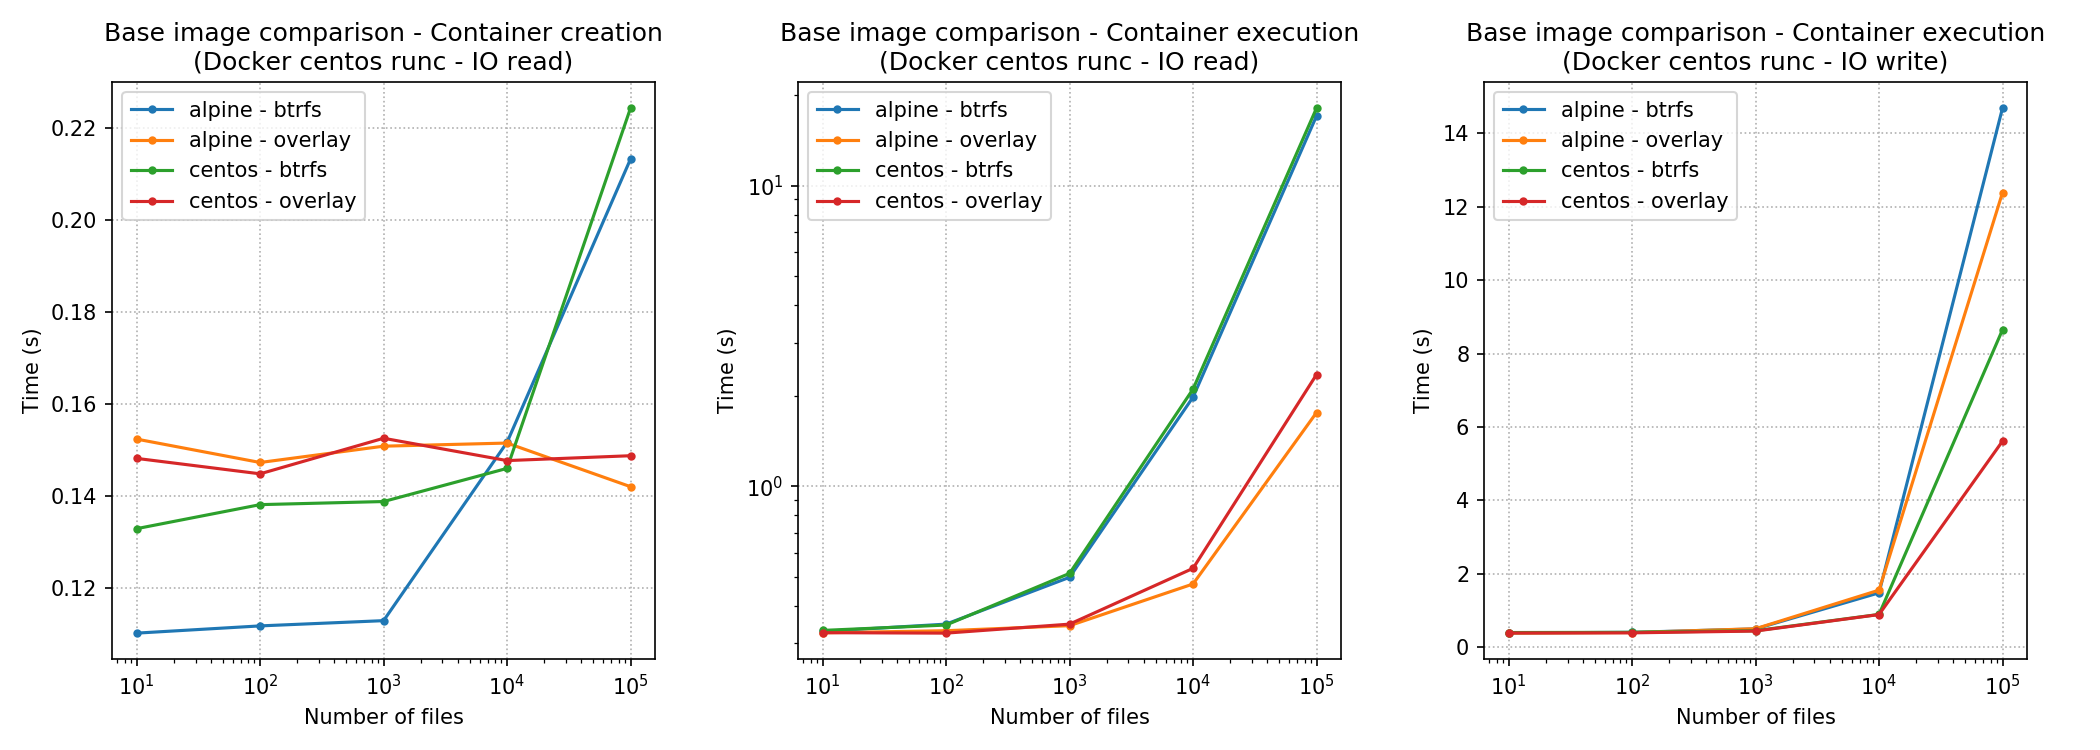
\includegraphics[width=\linewidth]{images/question-1-base-image.png}
    \caption{Base image performance comparison for containers launched with Docker and runc}
    \label{fig:q1:base-image}
  \end{center}
\end{figure}

From the graphs of Figure \ref{fig:q1:base-image}, we can notice several things:
\begin{itemize}
  \item We can see on the first graph (on the left) that, once more, btrfs offers better creation performances when the number of files is smaller.  Therefore, being a more complete linux distribution, with more functionnalities, and so, more files, Centos-based images are more costly for container creation.
  \item On the second graph, it also appears that simple read operations are a little bit faster when using Alpine as base image.  This trend has also been observed with bigger file read, with the \textit{Database read} test.
  \item One thing really interesting that we can see on last graph however, is that the trend seems to be inverted for write operations.  This difference is really likely to be caused by the difference in the implementation of \texttt{tar} (used for this test) in each distribution's package repository.  Indeed, the implementation coming from Alpine makes a lot more system calls (about three times more) than Centos's one.
\end{itemize}

The choice of Centos as base image can then be justified by the maturity of such distribution.  It had been around for a while, it is widely used outside of container applications, and is more likely to count optimization in the different tools at disposal.  If we don't require those tooles though, the minimalist and ligthweight aspect of Alpine makes it a better choice.

\subsubsection{Container runtime}

On Figure \ref{fig:q1:runtime} is chown the influence of different container runtime solutions on the different execution step of the container.  

\begin{figure}[h!]
  \begin{center}
    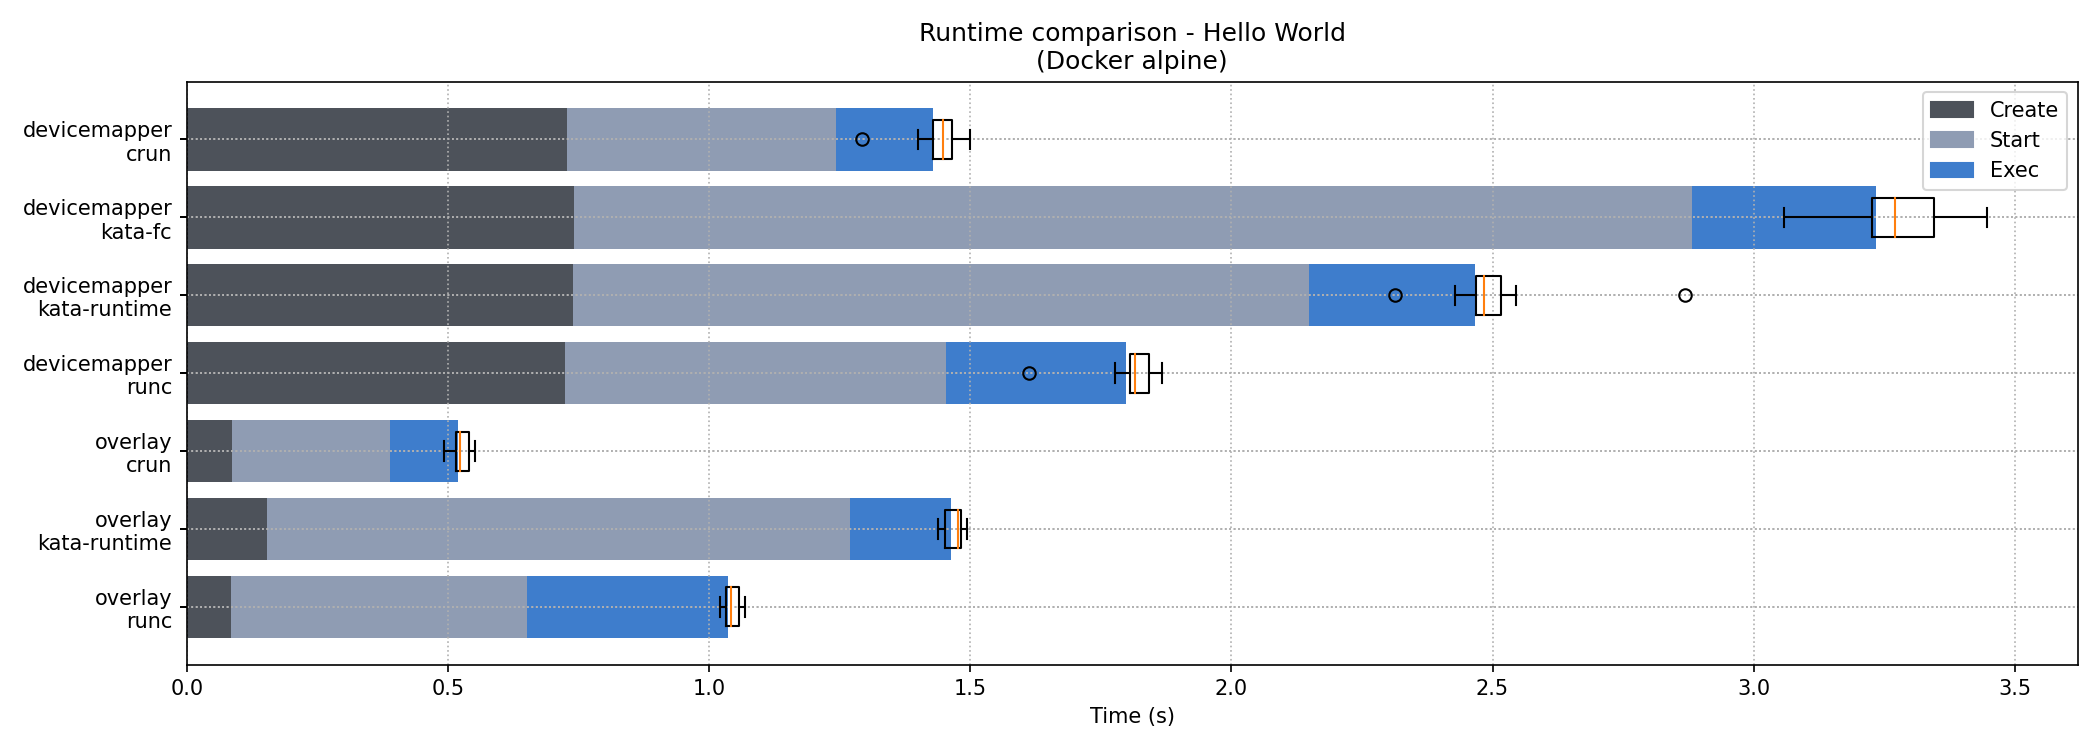
\includegraphics[width=\linewidth]{images/question-1-runtime.png}
    \caption{Runtime performance comparison for Alpine containers, launched with Docker}
    \label{fig:q1:runtime}
  \end{center}
\end{figure}

By first comparing crun to runc, we see how much of a difference it makes to use an efficient C implementation, over a less efficient Go one.  The difference is much more obvious for the \texttt{start} and \texttt{exec} phases as those are the steps where real low-level operations are made by the container runtime (entering namespaces, setting cgroups, forking processes).  

Then we have the Kata Containers solutions, based on virtualization.  It obviously will lead to a greater overhead for creating and starting containers, as a whole kernel as to be loaded.  However, the \texttt{exec} phase seem to have a much lower overhead.  We can't miss how much worse is \texttt{kata-fc} (using Firecracker hyperviser) compared to \texttt{kata-runtime}, and it might be disapointing given the recent popularity that has embrassed Firecracker.  In response to that here are some important elements:
\begin{enumerate}
  \item Firecracker has not been conceived to run under Kata Containers's hood.  It is really possible that it would perform better when running standalone.
  \item Some advantages that Firecracker has and that are not obvious in our study case are, first, the memory footprint, which is way smaller than with Qemu, and second, the reduced code base, which ensure a much lower attack surface.  Those are also reason why Firecracker is so popular.
  \item After some discussion with Kata Containers community\footnote{The full discussion can be found at this link: \href{https://github.com/kata-containers/runtime/issues/2642}{https://github.com/kata-containers/runtime/issues/2642}}, it turned out that Kata Containers make use of one feature of Qemu that Firecracker doesn't have, that would justify this difference in performance: vNVDIMM.  Thanks to vNVDIMM, the root file system of the guest VM is fully loaded in memory and directly accessed in it, which is faster than reading it from disk as Firecracker does.
\end{enumerate}

\subsubsection{Container manager}

On Figure \ref{fig:q1:manager} are shown the different container manager considered in the experiements, in the configuration that my tests revealed as most performant.  Docker and Podman using crun as runtime, and overlay or btrfs as storage driver.  LXD uses lxc as runtime and btrfs as storage driver.

\begin{figure}[h!]
  \begin{center}
    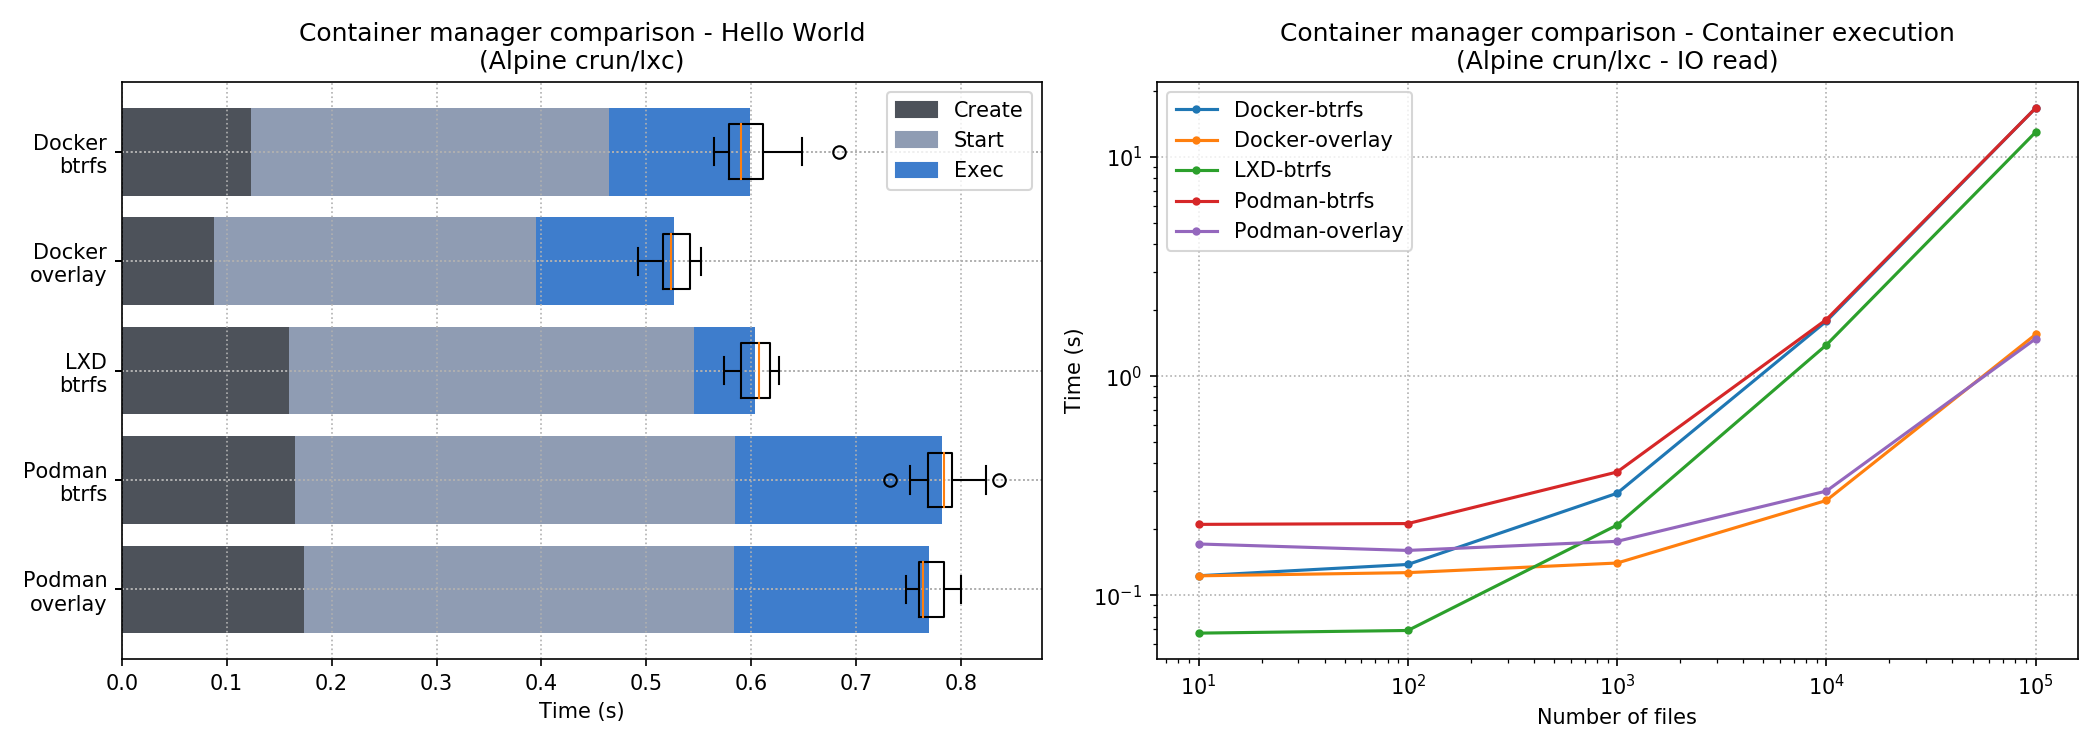
\includegraphics[width=\linewidth]{images/question-1-manager.png}
    \caption{Container manager performance comparison for Alpine containers}
    \label{fig:q1:manager}
  \end{center}
\end{figure}

We can see that Docker is still the best solutions for us, even though none of the other solution presents really bad performances.  Given the relatively young age of Podman, its focus might not be yet fully on performances, but rather on functionnalities, catching up all the things that the two other alternatives already have.  We can then hope for improvements on this side as time goes, it would be worth check on them later this year, or the next one.  

All those three solutions are reliable, have a great support, and a community to back them up.  LXD is maintained by canonical, which makes it a great fit for Ubuntu environments.  Docker is maintained by Docker Inc. and also seem to bring greater support for Ubuntu.  Podman is supported by the containers\footnote{\href{https://github.com/containers}{https://github.com/containers}} organization and is served as default Docker alternative on Fedora.  Using Podman on Ubuntu has been a bit more complicated than the two others, especially for the rootless solution, which requires cgroupv2.  Thankfully the community offered great support for all of my problems, and in most cases the issues appeared to be with systemd or Ubuntu, rather than with Podman.

\subsubsection{Final configuration}

Based on the previous observations, the ideal configuration would then be:

\begin{center}
\begin{tabular}{rl}
  \textbf{Container manager} & Docker \\
  \textbf{Base image} & Alpine/Centos \\
  \textbf{Storage driver} & overlay2 \\
  \textbf{Container runtime} & crun \\
  \textbf{Control group version} & v1 \\
  \textbf{Rootless containers} & no \\
\end{tabular}
\end{center}

As we can see, the final configuration is not that much different from the original one.  The quick answer to the original questions would be:
\paragraph{}\textit{Compared to other available solutions, how good is the current configuration chosen by INGInious to face the responsiveness challenge of the platform?}  The current configuration is good.  It could be improved, but is definitely not the worse one.  The choice of going with Docker was the most soundfull when INGInious was created, and it is still the case now.  The current storage driver offers great performances for almost every cases, only some specific case, sollicitating a lot of IO operations on big files, can give an advantage to another storage driver, btrfs.  The choice of a Centos base image is not bad either, but the size of the image being greater than Alpine's one, except for the situations where Centos offered better write performances, using Alpine seems to be better.  The move here might then be to go for an hybrid solution, using Centos only in situations where its small writing performance advantage become meaningfull.  
\paragraph{}\textit{How much better could it be?}  As we have seen, changing the current container runtime makes a significant difference.  The c implementation of \texttt{crun} is claimed to be twice as fast as the go implementation of \texttt{runc} by \texttt{crun}'s contributors.  And we can definitely see the difference.  The change of base Image though doesn't show as obvious improvement.
\paragraph{}\textit{How easy would it be to improve it?}  This is the real good news, it truely is super easy to apply the most significant change.  You only need to install \texttt{crun}, reconfigure Docker to use it by default, and you are good to go, no change as to be done to INGInious!  For the base of the base image the story is different though, as it would require to change all the containers images, which is a lot of work.

\section{INGInious ideal solution}
We will here consider the second question:
\begin{center}
  \say{\textit{Could there be a solution tailor-made for the specific case of INGInious?  What would it be?  What would it cost to use it?}}
\end{center}

The different container manager presented here are very versatile solutions, they all have a great package of functionnalities that allows them to deal with a wide range of different applications.  This is good for them, but bad for us, as we don't need most of those functionnalities, but still pay the cost through a more heavy container manager.

The workload that INGInious handles with its container manager is not that extensive, it is actualy even quite redundant, and predictible, as each student's code is expected to have a specific behavior.  And that expected behavior can actually define in advance, which files in the container filesystem are going to be modified, and which aren't.  We can play with that knowledge.

I have then created a small concept alternative solution, that would just fit the needs of INGInious, and provide better performances.  It relies on two things:
\begin{enumerate}
  \item We don't need a fully functionnal and grown up container manager. Our needs are simply containers, with resource management.  Those are provided by tools like crun and runc and cgroup v1 and v2.  We could then gain performance by only using those.
  \item We don't need a complete writable filesystem for each container, we can restrict write access to certain parts of it.  Which means that we could copy the file that will be modified, when creating the container (avoiding the need of using any copy-on-write mechanism), and bind-mount the rest of it, with read-only permissions.
\end{enumerate}

\begin{figure}[h!]
  \begin{center}
    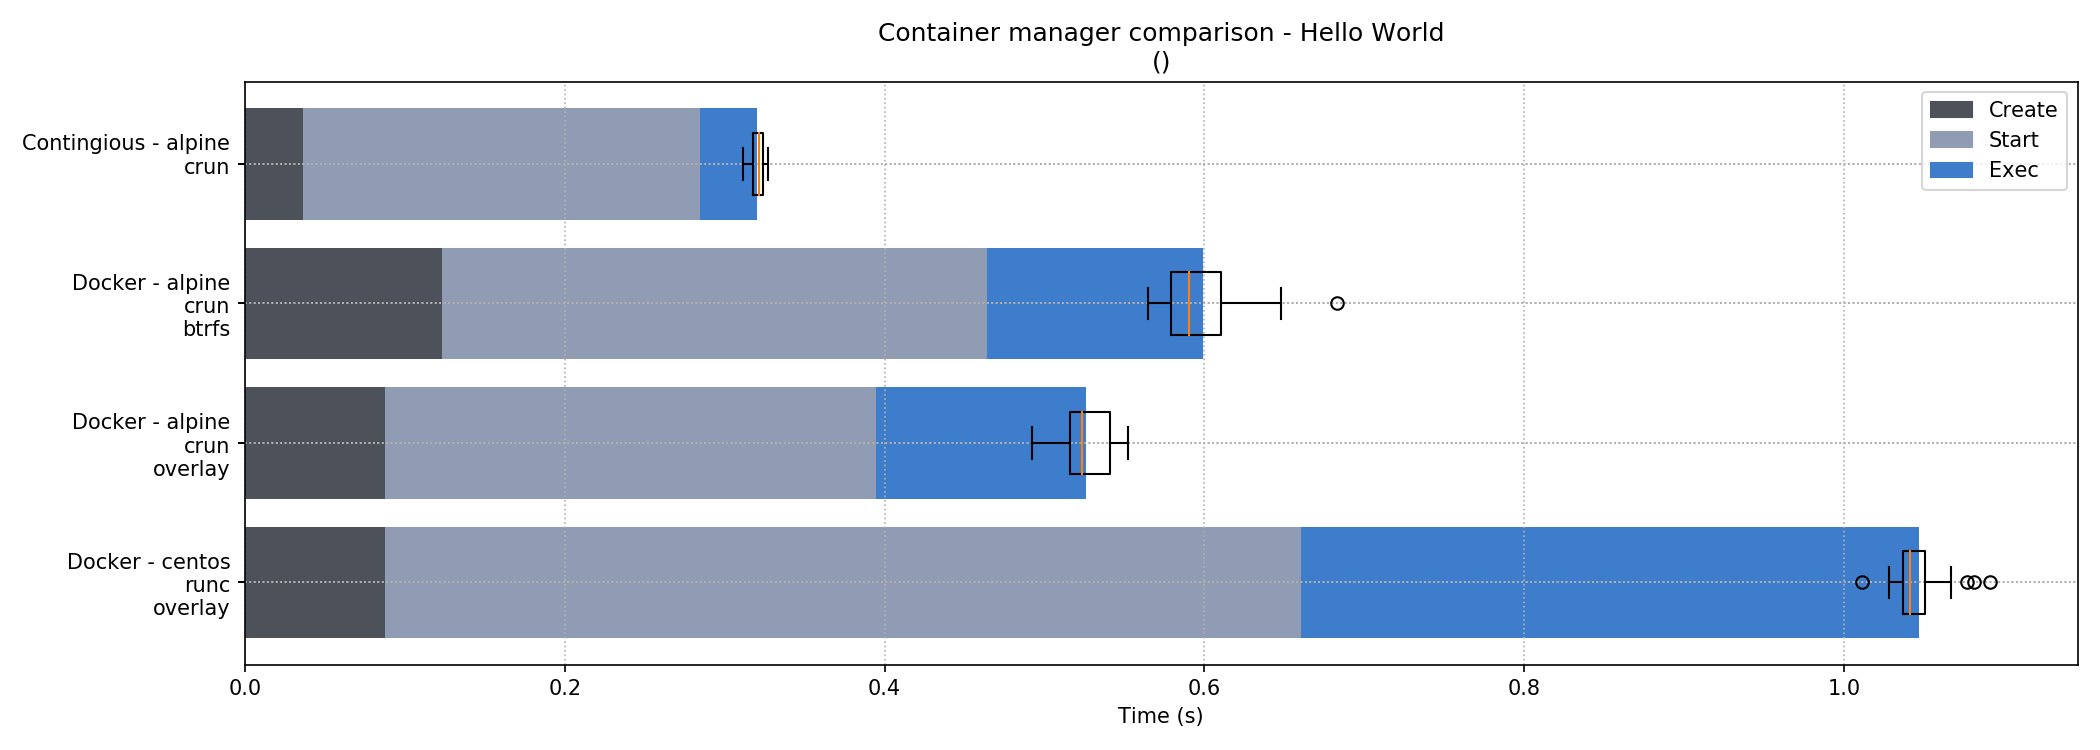
\includegraphics[width=\linewidth]{images/question-2-hello-world.png}
    \caption{Ideal INGInious container manager solution compared to the current configuration of the platform and to the recommended new solution, Hello World test}
    \label{fig:q2:hello-world}
  \end{center}
\end{figure}

On Figure \ref{fig:q2:hello-world} we can see that the gain in performance is real, and we didn't give up any of the key requirement of INGInious.  We have the same level of isolation that Docker provides as we rely on crun, we even made it one step further as this solution is completely rootless.

\begin{figure}[h!]
  \begin{center}
    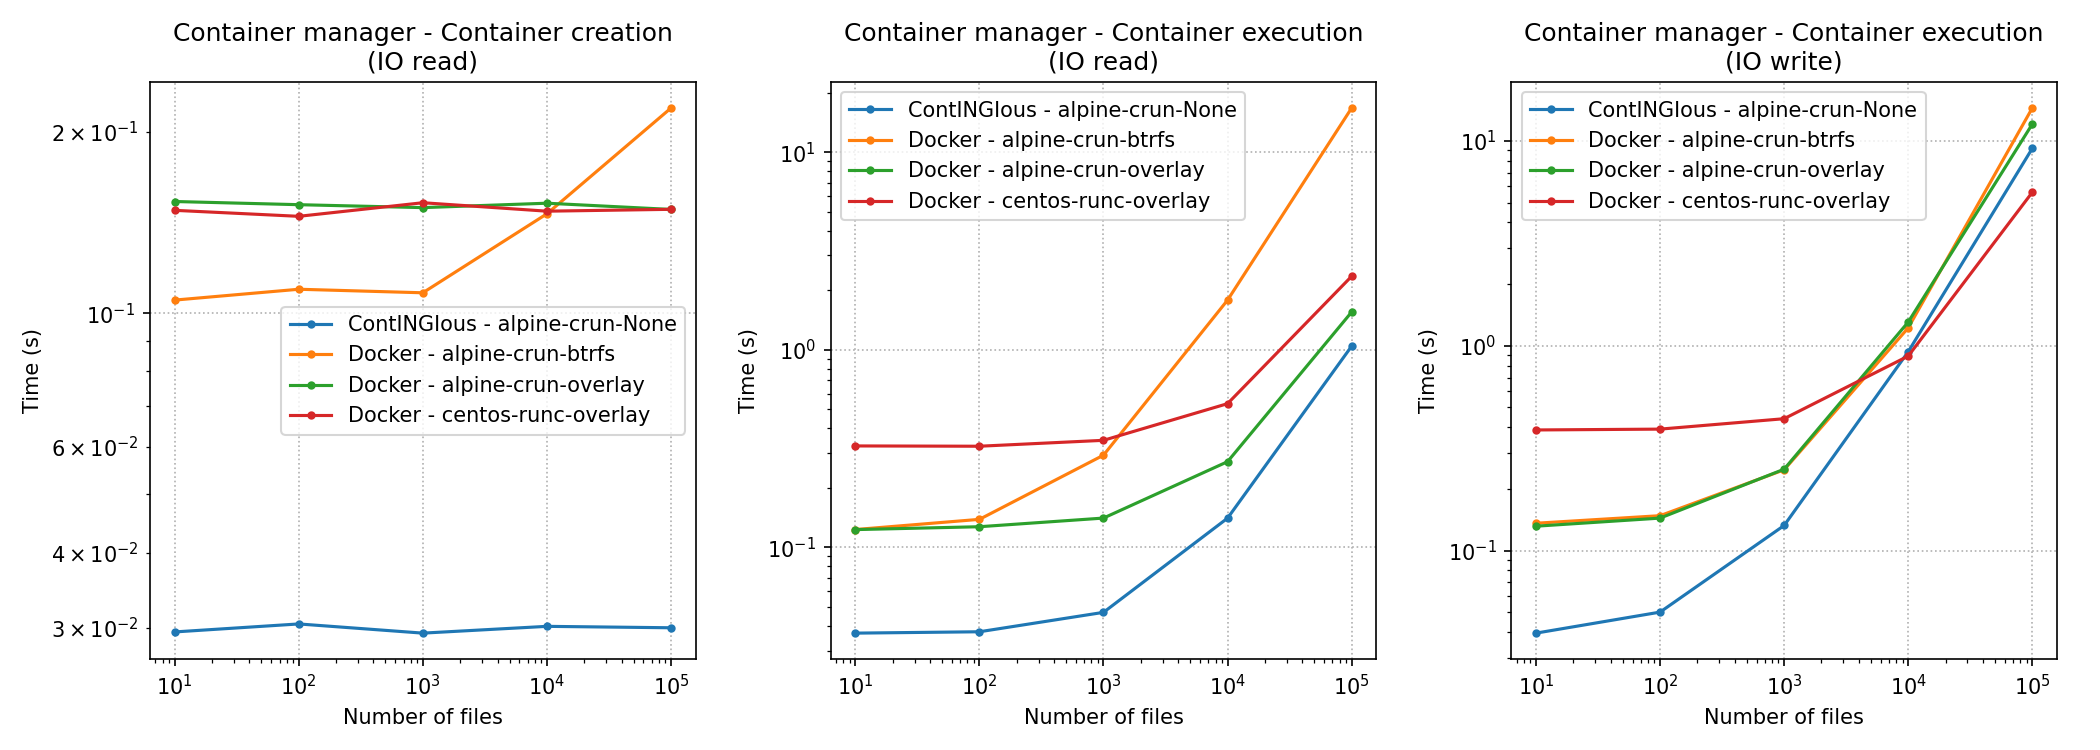
\includegraphics[width=\linewidth]{images/question-2-io.png}
    \caption{Ideal INGInious container manager solution compared to the current configuration of the platform and to the recommended new solution, IO tests}
    \label{fig:q2:io}
  \end{center}
\end{figure}

On Figure \ref{fig:q2:io} we can see that the only battle we loose is with the current INGInious solutions for the write test, as its \texttt{tar} implementation is more efficient.  Otherwise, reading file is way fatser when you don't need to manage differet layer of your file system as with overlay, and writing is faster too as, again, we don't need to care about different layers.

\begin{figure}[h!]
  \begin{center}
    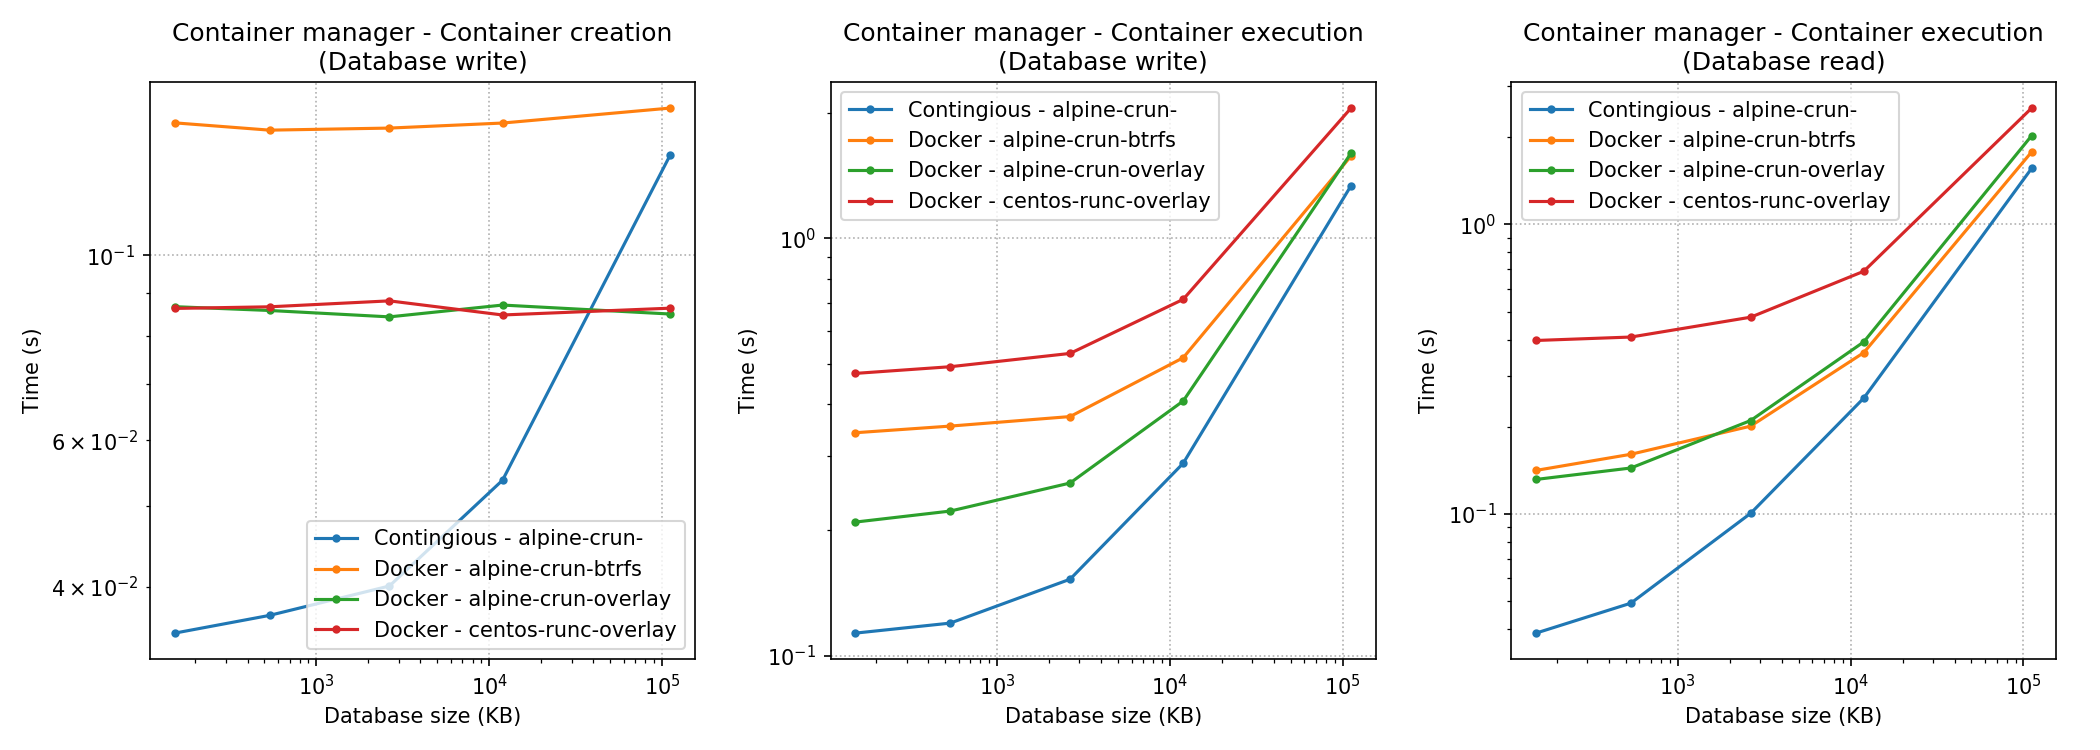
\includegraphics[width=\linewidth]{images/question-2-db.png}
    \caption{Ideal INGInious container manager solution compared to the current configuration of the platform and to the recommended new solution, Database tests}
    \label{fig:q2:db}
  \end{center}
\end{figure}

On Figure \ref{fig:q2:db} we see that this solution isn't magical though, copying file before editing them is still costly.  But doing this when creating the container still provides overal better performances than copying the file to a higher layer as overlay just before writing it.  The only alternative that could beat us for more extreme situations are block-based copy-on-write solutions, as they won't copy the whole file.  That being said, we could probably improve this solution by making use of that feature too, relying on an underlying filesystem that has such capabilities.

\paragraph{}Here we have a solution tailored-made for INGInious then.  But it doesn't mean we should actually use it.  What I presented here was a working prototype, not a realiable solution, a lot of work has still to be done to make it work easily and integrate it into INGInious.  Among that work you can count the following things:
\begin{itemize}
  \item Determine for each container which should be the writable part of the file system.  And eventually optimize those images by centralizing all the writable content.
  \item Create a new image management system.  We don't need to go from scratch though, Buildah\footnote{Buildah is a tool that allows to easily build and manage OCI images. \href{https://github.com/containers/buildah}{https://github.com/containers/buildah}} could be used, and would even allow us to continue using Docker Hub to store images.
  \item Integrate all the mangement of the steps of creation and execution of containers in one reliable tool.  For that we don't need to start from scratch, it might be worth taking a look at conmon\footnote{Conmon is the container runtime monitor on which podman rely.  \href{https://github.com/containers/conmon}{https://github.com/containers/conmon}}.
\end{itemize}

Whether the performance improvement of this solution is worth the effort it would require is not my call to make. I like that idea, and think it would make a great project, but I would also cost a lot of time to set up and maintain.

\section{INGInious opportunities}
We will here consider the last question:
\begin{center}
  \say{\textit{What would be the cost of providing a stronger/safer isolation to the containers used by INGInious?  What opportunities could it bring?}}
\end{center}

By saying "\textit{providing a stronger-safer isolation}" what I mean is more mitigating the risk we take when we let a student execute code in a container, on the host where the platform is running.  The most unsafe solution (still making use of containers) is to run the container as root, with the root user of the container in the hand of the student, and mapped to the root of the host.  In theory this doesn't do any harm, but given past vulnerabilities that have been found in runc it can happen.  To mitigate this, INGInious currently creates a new user in the container, which has no root priviledge (neither inside the container nor outside of it), for the student code to execute.  This limits the range of possibilities of task to evaluate with INGInious.  We cannot for example simulate a cluster of machine where the student has root access in order to deal with any network assignment.

\subsubsection{Rootless containers}
\paragraph{}The first possibility to improve this situation is to go with rootless containers.  We have two alternatives for this: Podman's rootless containers and LXD unpriviledged containers.  Docker is also working on a solution but has only limited support for now.  With rootless containers, not only the root inside the container isn't root on the host, but also the container runtime isn't running as root, which limits a lot the damage that can be done to the infrastructure if a vulnerability in the container runtime is found and exploited.  It also mitigate potential attacks the other way arround, for a user on the host that would try to gain root access through a vulnerability of the container manager.  This is only valid for Podman though, as LXD's daemon is running as root, even for unpriviledged containers.  Podman could then be installed on student's machine in computer rooms without too much concern.

\begin{figure}[h!]
  \begin{center}
    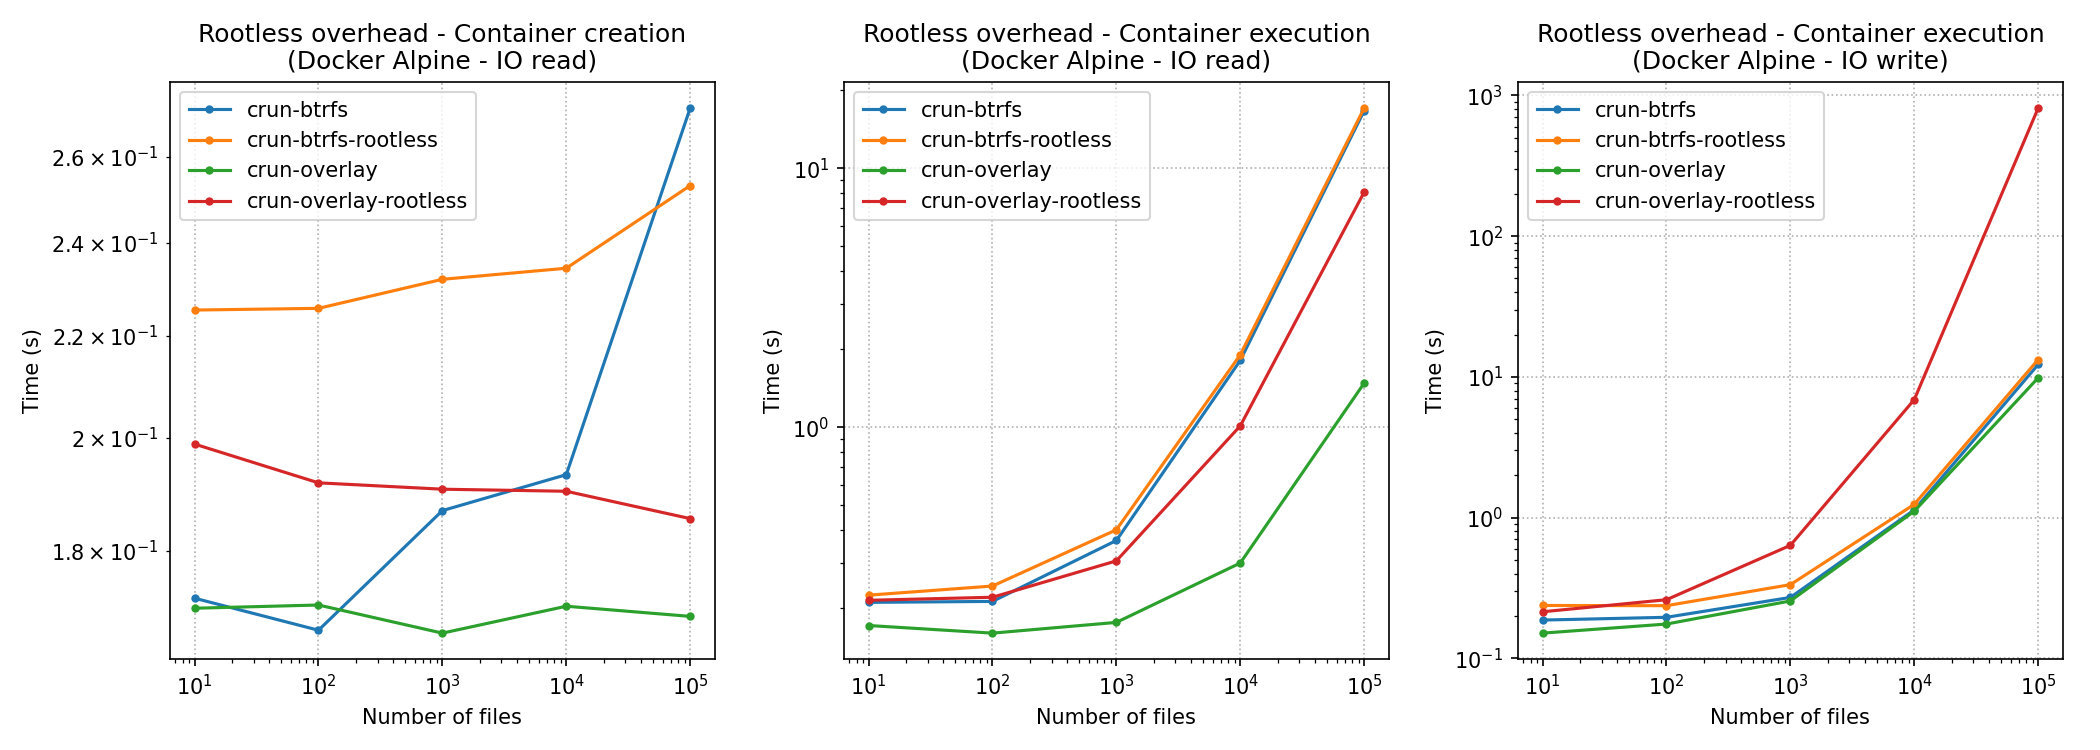
\includegraphics[width=\linewidth]{images/question-3-rootless-io.png}
    \caption{Overhead of rootless containers compared to rootfull ones, IO tests}
    \label{fig:q3:rootless:io}
  \end{center}
\end{figure}

Unfortunetly, having rootless containers also comes with a cost as we can see on Figure \ref{fig:q3:rootless:io}.
\begin{itemize}
  \item There is a cost to create, start and execute command into rootless containers with Podman compared to going rootfull with the same container manager.  This is very likely caused by the extra steps required to be taken to launch rootless container with all the functionnalities of a rootfull one.  Podman needs first to unshare user and mount namespaces, to be able to make bind mounts on the container filesystem.  It also requires to add a cgroup scope to all the commands that setup the containers, to be sure that the container runtime will later be able to move process created to the cgroup attached to the container.
  \item Because of the lack of \textit{real} root permissions on the machine, rootless containers can not use OverlayFS, instead they use a fuse implementation of the latest, which, as we can see on the right-most graph, induces great performances cost.  It get even worse when doing write operations.
  \item One limitation of rootless container is also the options available for managing the storage of containers (storage drivers), for example devicemapper isn't available.
\end{itemize}

\subsubsection{Virtualization}
\paragraph{}Another solution is to simply strengthen the isolation that protects the host from the student.  And the best solution to do this is to make use of virtualization.  Kata Containers is a great deal for us, it allows us to keep the infrastructure of the platform, only changing the runtime used by Docker, and everything can still be used as before.  Once again, this stonger isolation level could open the gate to assignements that would require for the student to have root access in the container.

\paragraph{}However, as we already saw earlier when comparing runtimes, virtualization adds a cost, mainly to container startup, but also on creation and execution.

On Figure \ref{fig:q3:virtualization:io}, we can notice that unlike for crun, the overlay storage driver behave way worse than devicemapper.  This is actually also the case for all other storage drivers too, it seems that runtime solutions with virtualization take much more advantage of devicemapper than other drivers.  And passed a certain point, Kata Containers using Qemu even perform better than crun, both in read (compared to crun with devicemapper) and write (compared to crun with overlay or devicemapper).

\begin{figure}[h!]
  \begin{center}
    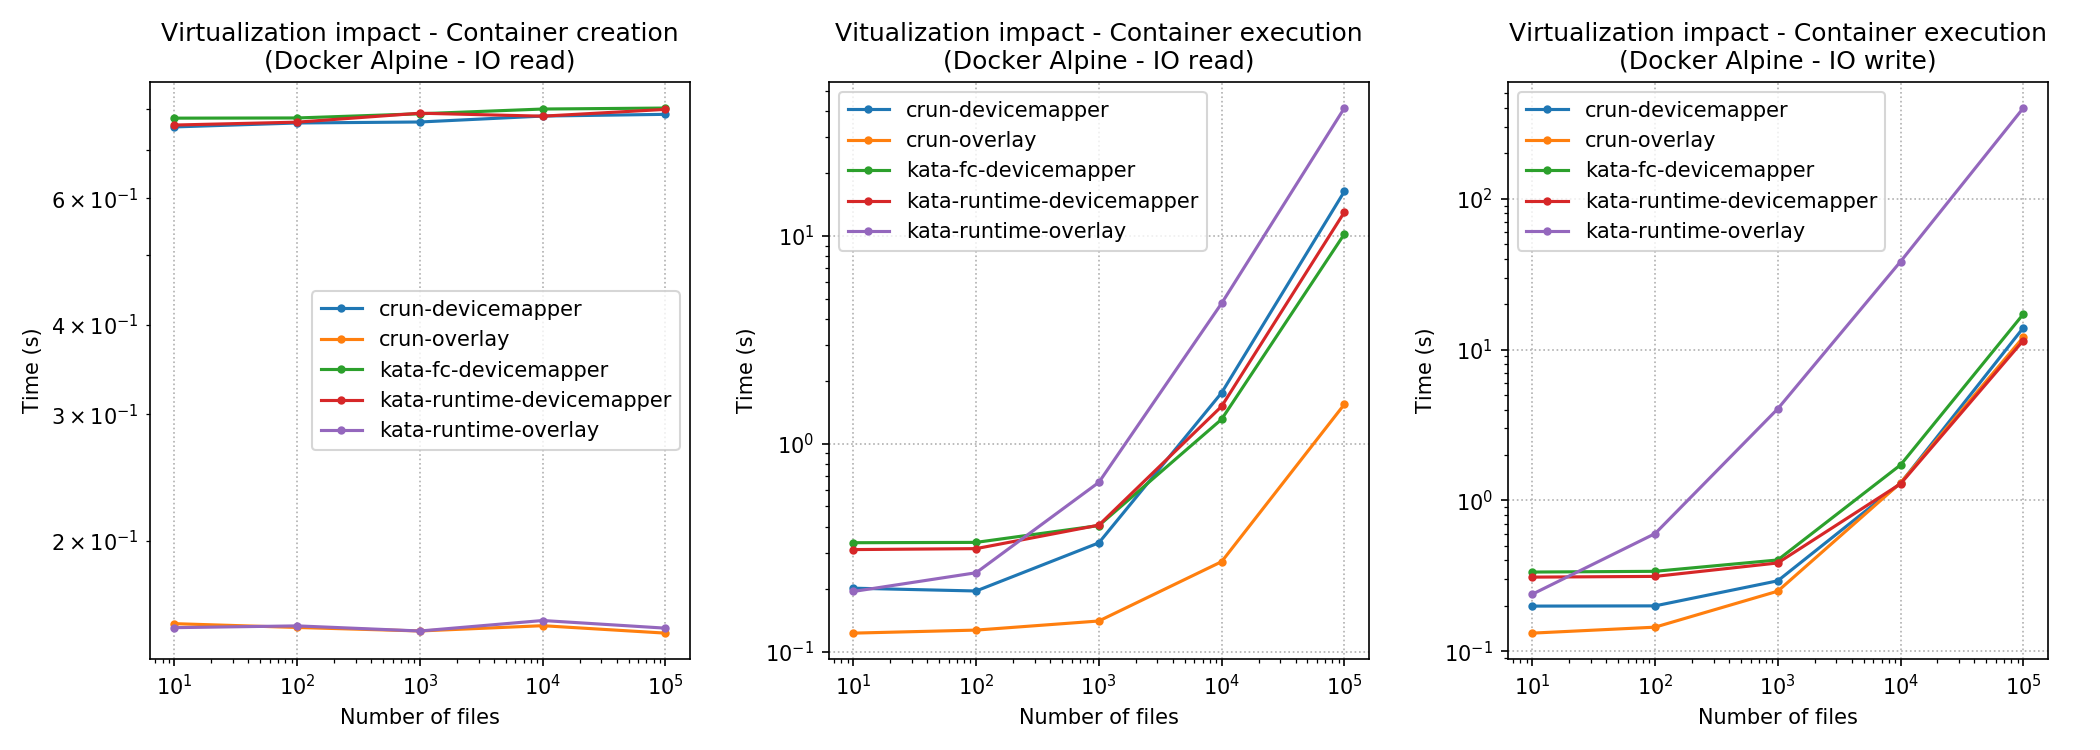
\includegraphics[width=\linewidth]{images/question-3-virtualization-io.png}
    \caption{Cost of virtualization on container creation and execution, IO tests}
    \label{fig:q3:virtualization:io}
  \end{center}
\end{figure}

We can make the same observation on Figure \ref{fig:q3:virtualization:db} with the excpetion than, for some reason, Kata Containers using Firecracker seems to handle read operations on big files much better than when using Qemu.

\begin{figure}[h!]
  \begin{center}
    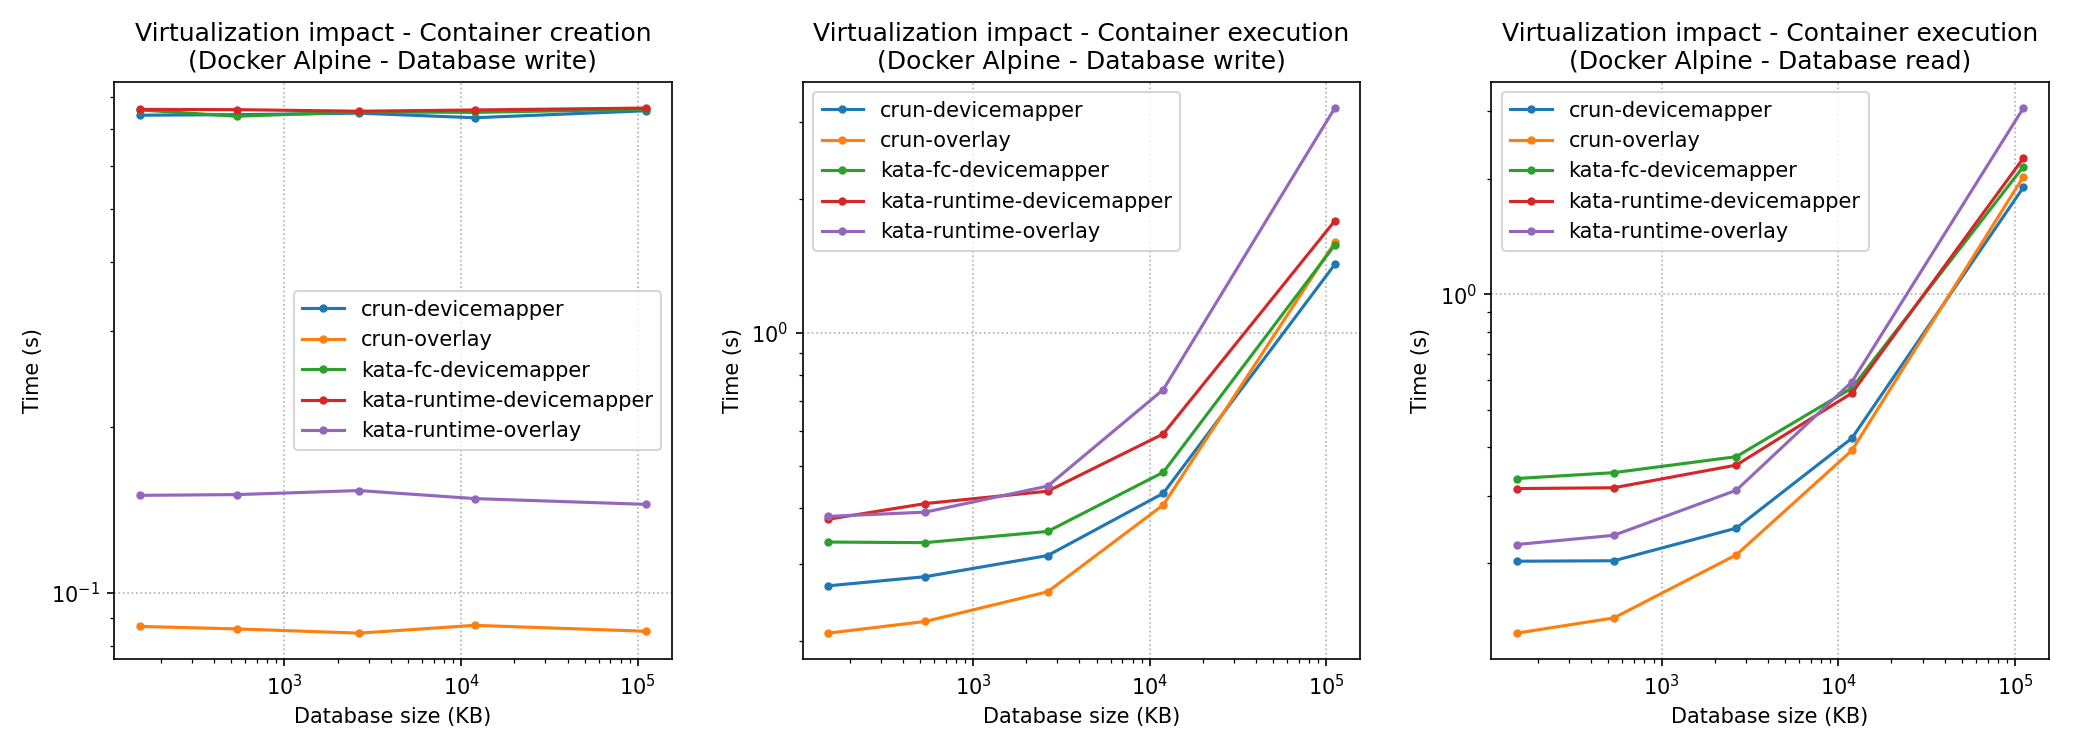
\includegraphics[width=\linewidth]{images/question-3-virtualization-db.png}
    \caption{Cost of virtualization on container creation and execution, IO tests}
    \label{fig:q3:virtualization:db}
  \end{center}
\end{figure}

One more great thing about Kata Containers is that every container in the same pod (group of containers, linked together, that serves a common global purpose) will actually be grouped inside the same vm (still in separate containers), this will reduce the overhead by container caused by virtualization as the size of the pod grows.  This could be convenient for assignment where multiple containers needs to be managed by a single student.  Unfortunetly, to make use of this feature, the container manager needs to have some kind of pod mechanism, which isn't the case of Docker.  Podman, Kubernetes or others can do that.

  \chapter{Conclusion}

  
  \appendix
  \chapter{Container life cycle} \label{appendix:container-life-cycle}
During its life cycle, a container will go through five stages: creation, launch, execution, stopping and cleaning.  Those five steps are explained below and presented in figure \ref{fig:container-life-cycle}, along with the corresponding command for each presented tool.  Other optional stages (like pause/unpause) are not presented here.
\begin{enumerate}
\item\textbf{Create} This is the set-up phase, depending on the tool, the file system of the new container might be copied, or any other things that need to be done before launching the container.  This phase can only be done one time for each container.
\item\textbf{Launch} This is the proper instantiation of the container, the namespaces are created, the new file system is adopted.  Depending on the container, a complete init process might be executed.  This state can be repeated as many times as we want for a container, as long as it is in a stopped state.
\item\textbf{Execute} This corresponds to the execution of a process in the container.  This can be done as many times as we want for a container, as long as the container is running.
\item\textbf{Stop} This is when the container needs to be stopped, all running processes are killed, and the namespaces are exited.  No modification should be done on the filesystem, the storage of the container remains.
\item\textbf{Clean} This is the un-create phase, where we delete everything that was done during the creation phase.  The storage will be lost after this phase.
\end{enumerate}
\begin{figure}[!h]
  \begin{center}
    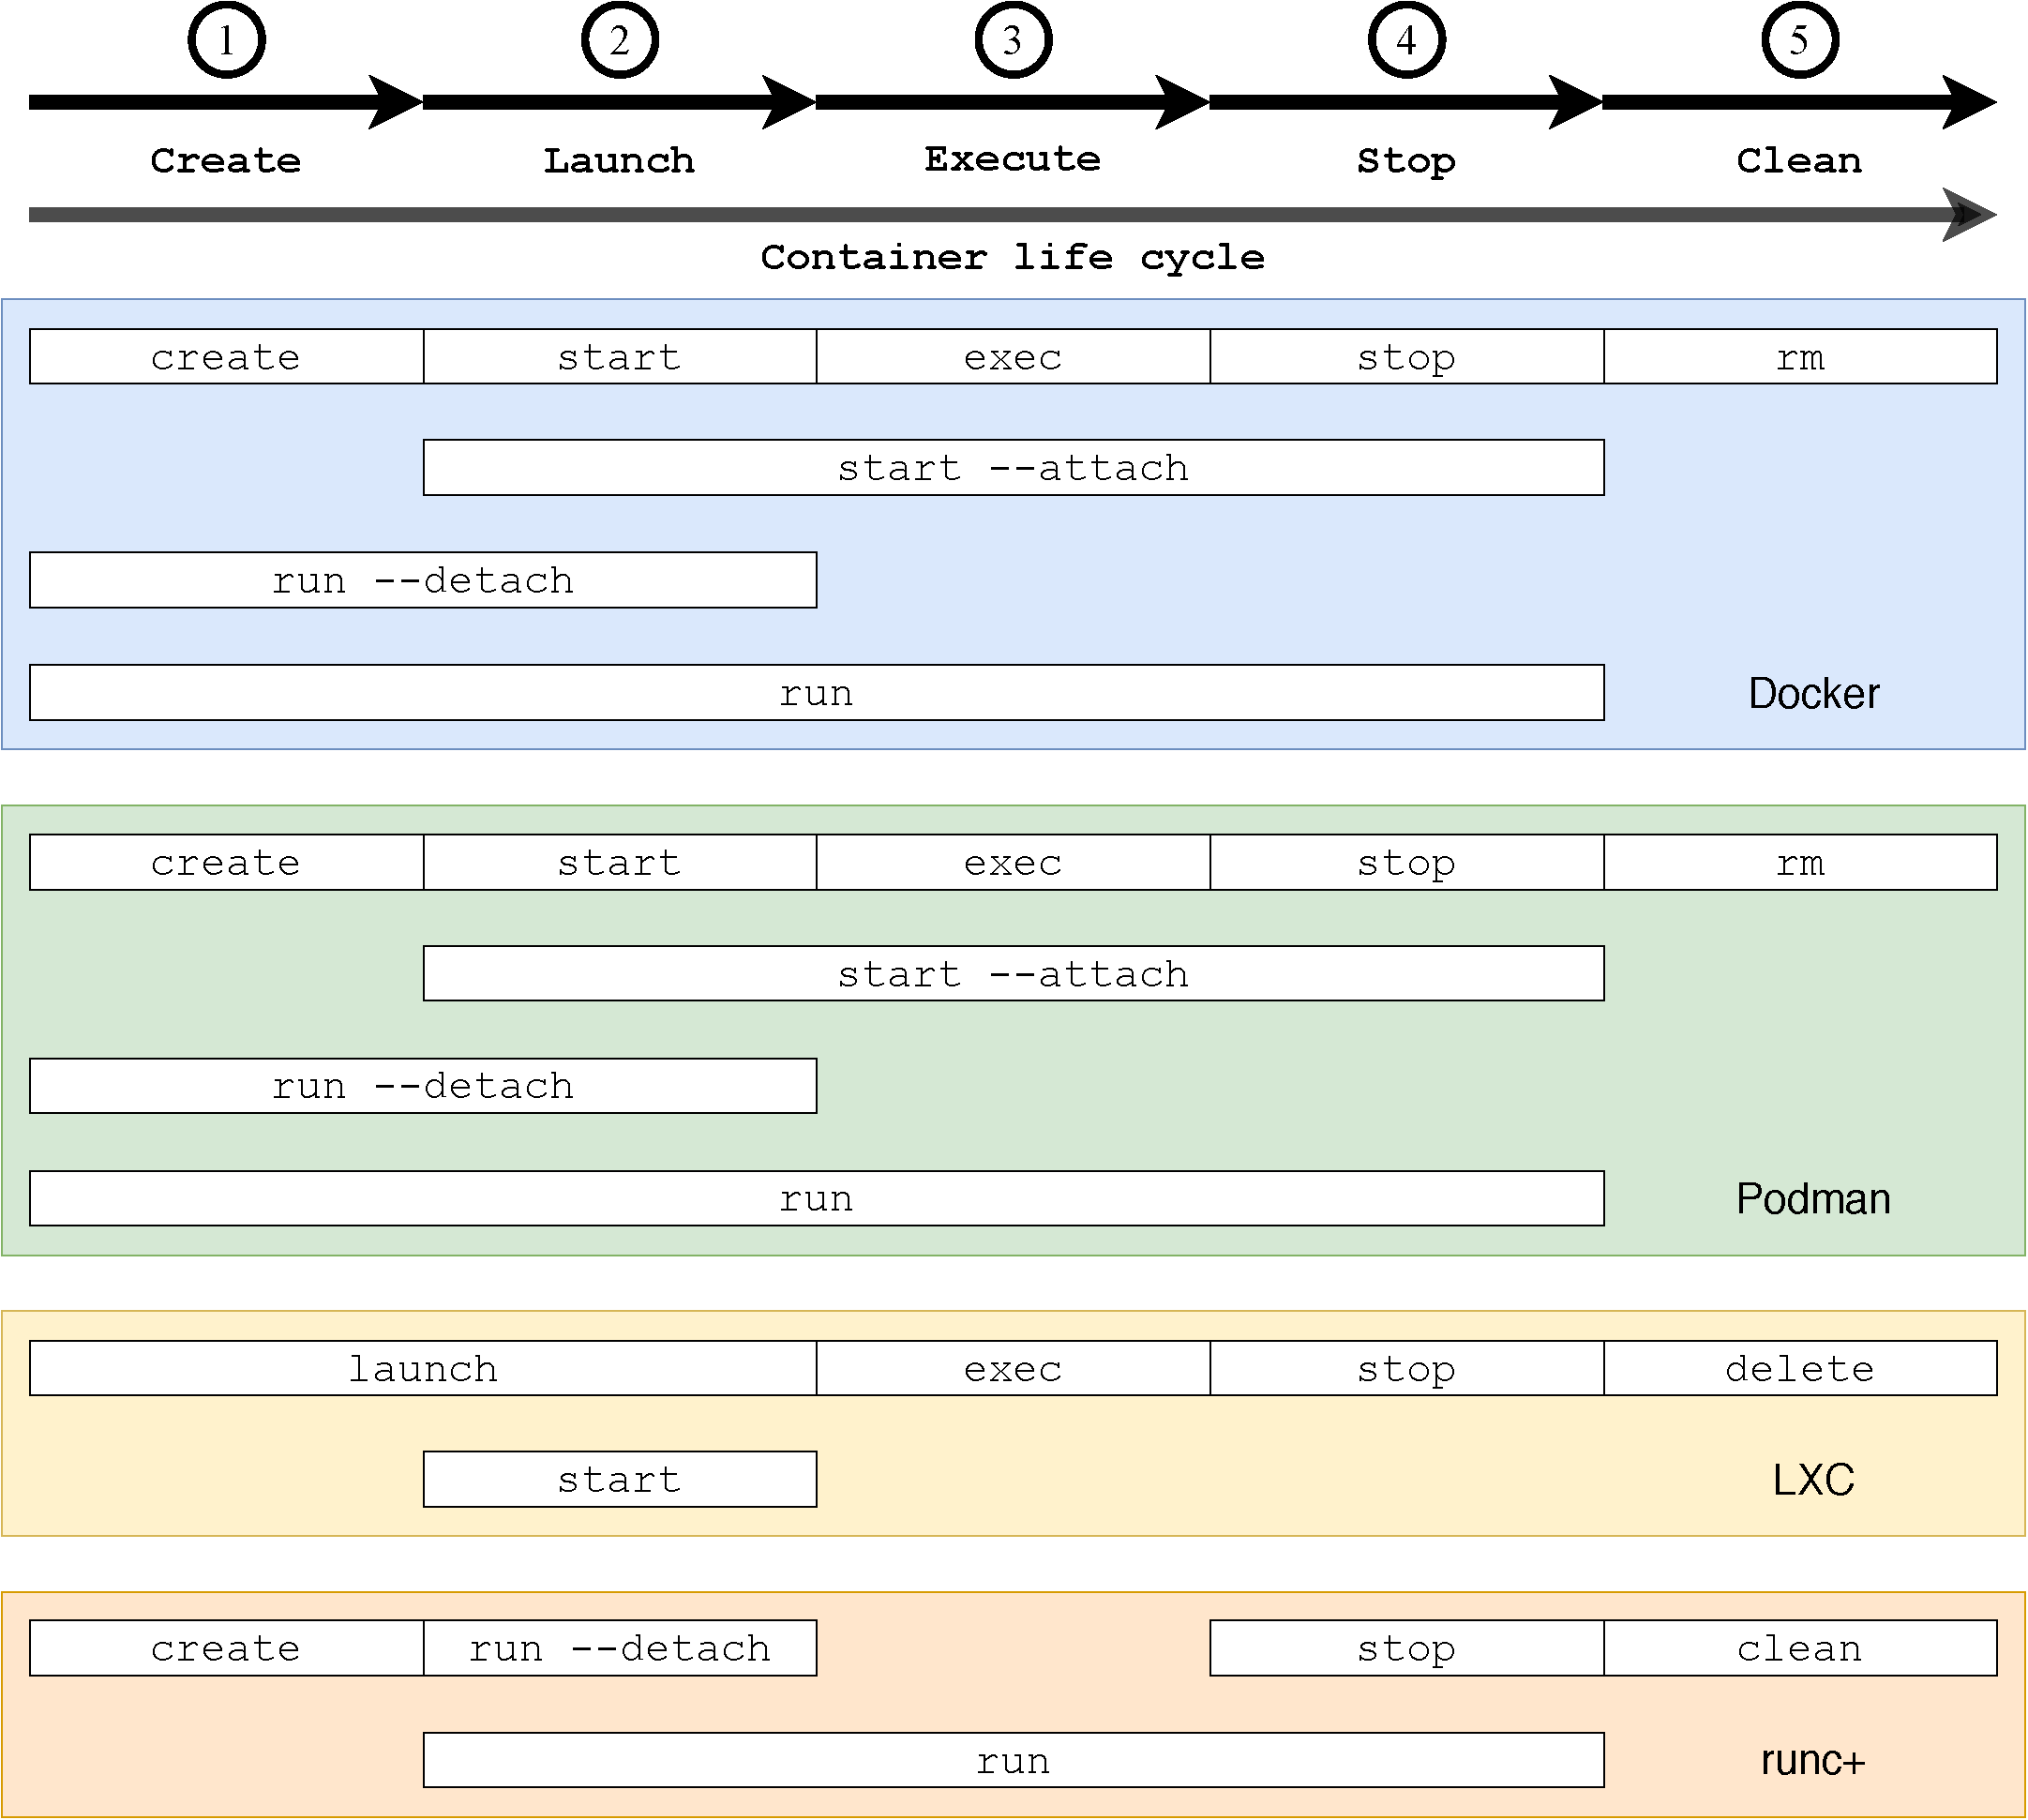
\includegraphics[width=\linewidth]{images/Container-life-cycle.pdf}
    \caption{Container life cycle and how to interact with it.}
    \label{fig:container-life-cycle}
  \end{center}
\end{figure}

  
  \bibliography{bibliography}{}
  \bibliographystyle{plain}

  % Back cover page
  \backcoverpage

\end{document}
